\documentclass[]{article}

\usepackage{xcolor,listings}
\usepackage{textcomp}
\lstset{upquote=true}

\usepackage{polski}
\usepackage[utf8]{inputenc}

\definecolor{lightblue}{RGB}{0,200,255}
\definecolor{lightg}{RGB}{240,240,240}


\usepackage{geometry}
\geometry{
	a4paper,
	total={170mm,267mm},
	left=20mm,
	top=15mm,
}


\usepackage{lscape}
\usepackage{pdflscape}
\usepackage{rotating}
\usepackage{epstopdf}
\usepackage{float}
\usepackage{amsmath}
\usepackage{amsfonts}
\usepackage{amssymb}
\usepackage{graphicx}
\usepackage{tabularx}


%opening
\title{Podstawy baz danych\\Projekt i implementacja systemu bazodanowego}
\author{Józef Jasek \\ Arkadiusz Placha}
\date{}

\begin{document}

\maketitle

\section{Opis systemu}
Firma organizuje konferencje, które mogą być jedno- lub kilkudniowe. Klienci, którymi są firmy lub osoby prywatne rejestrują się przez serwis www. Muszą podać listę uczestników nie później niż 2 tygodnie przed rozpoczęciem konferencji/warsztatu. Dla konferencji kilkudniowych uczestnicy mogą rejestrować się na dowolne z tych dni. Z poszczególnymi dniami konferencji związane warsztaty, na których uczestnictwo jest możliwe tylko w przypadku uczestnictwa w odpowiednim dniu konferencji. Warsztaty mają stałą cenę, a dni konferencji różne w zależności od momentu zarezerwowania sobie miejsca. W obu sytuacjach liczba miejsc jest ograniczona. Klienci mają tydzień na dokonanie płatności, inaczej rezerwacja jest anulowana. Baza danych dostarcza organizatorowi zbiór najważniejszych danych takich jak listy osobowe uczestników na dany dzień, czy warsztat lub informacje o klientach korzystających najczęściej z jego usług. Baza dostarcza danych, które są wyświetlane użytkownikowi, przyjmuje również wszelkie informacje o dokonywanych rejestracjach, płatnościach itd.

\begin{landscape}
	\section{Schemat}
	\begin{figure}[H]
		\centering
		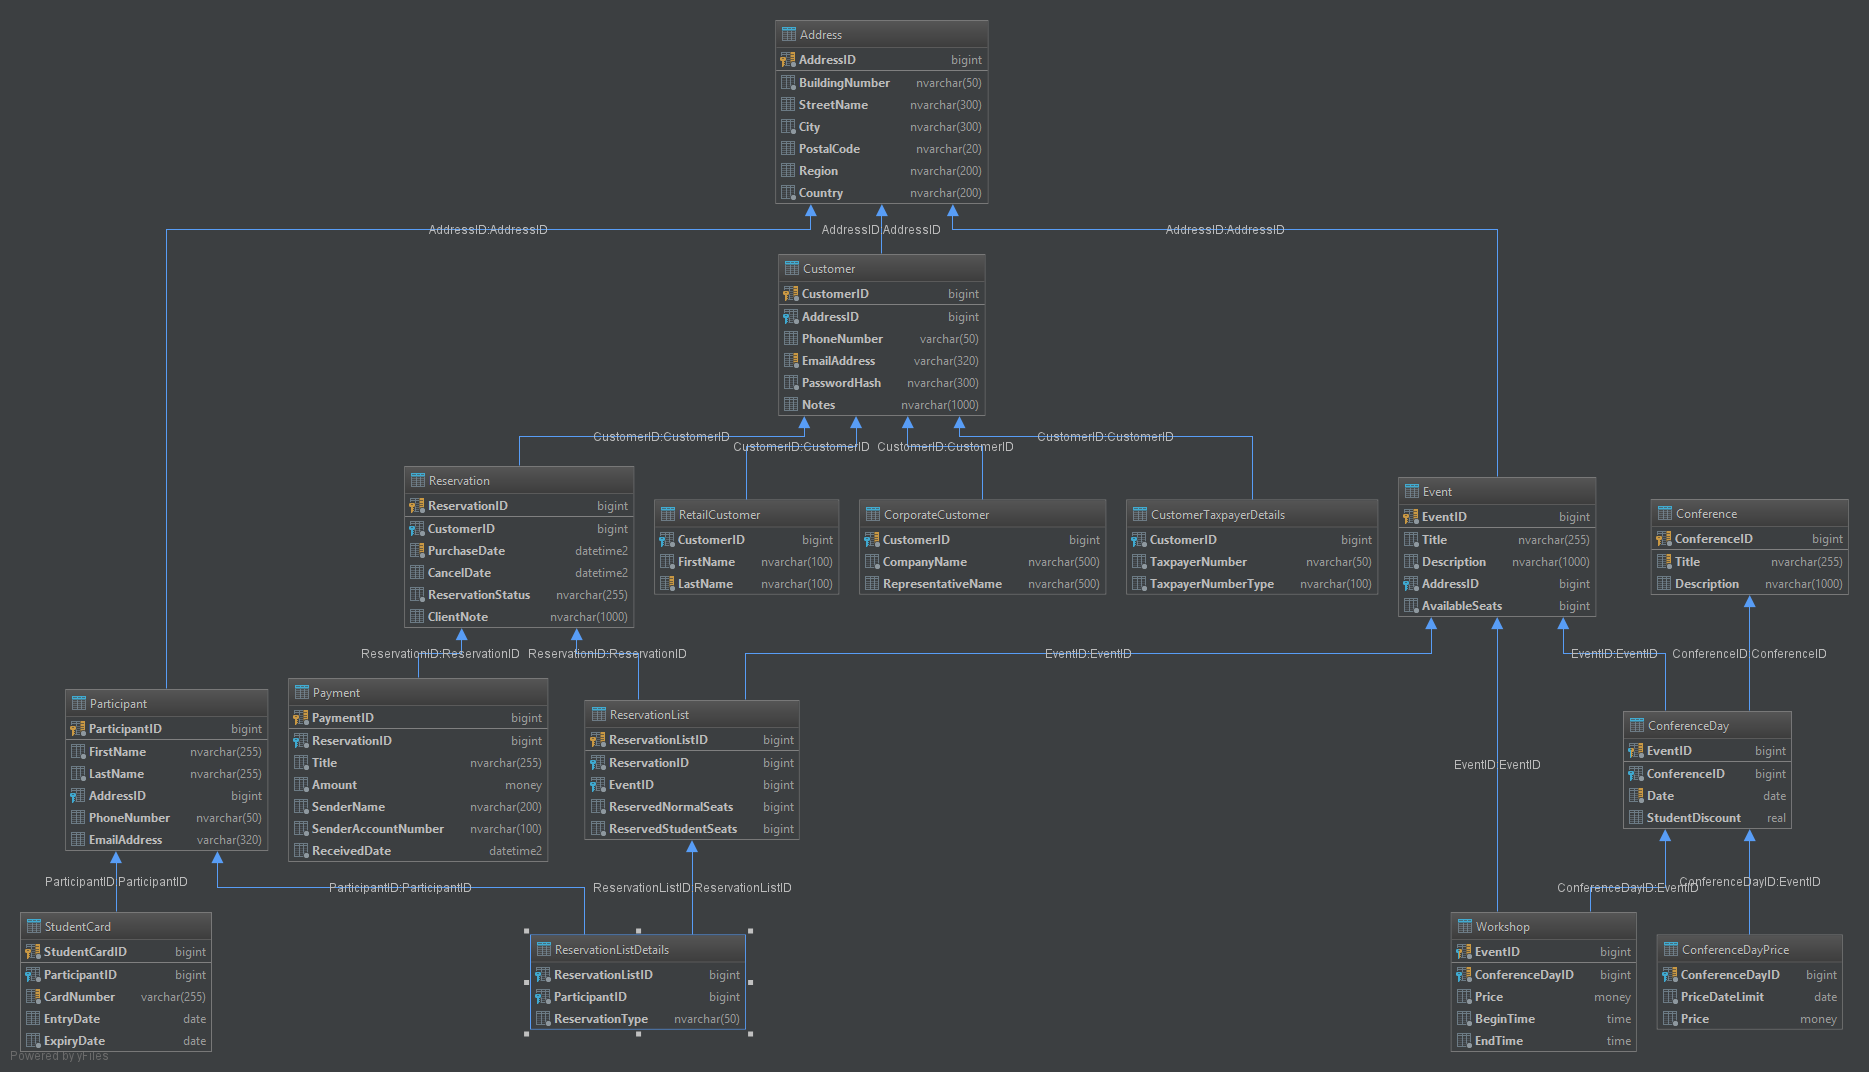
\includegraphics[height=0.8\textheight]{database}
	\end{figure}
\end{landscape}

\section{Opis tabel}
	\subsection{Address}
	Tabela przechowująca adresy zamieszkania klientów bądź wydarzeń. Adres składa się z (ID, nr budynku, ulica, miasto, kod pocztowy, region, kraj).
	\begin{lstlisting}[language=SQL,
						showspaces=false,
						basicstyle=\ttfamily,
						numbers=left,
						numberstyle=\tiny,
						backgroundcolor=\color{lightg},
						keywordstyle=\color{lightblue},
						commentstyle=\color{gray}]
create table Address
(
	AddressID bigint identity
	constraint PK_ADDRESS
	primary key,
	BuildingNumber nvarchar(50) not null,
	StreetName nvarchar(300),
	City nvarchar(300) not null,
	PostalCode nvarchar(20),
	Region nvarchar(200),
	Country nvarchar(200) not null
)
go

		\end{lstlisting}
	\subsection{Conference}
	Tabela przechowuje nazwę i opis konferencji. Przyporządkowane są do niej odpowiednie dni konferencji, skąd można odczytać jej datę rozpoczęcia i zakończenia.
	\begin{lstlisting}[language=SQL,
						showspaces=false,
						basicstyle=\ttfamily,
						numbers=left,
						numberstyle=\tiny,
						backgroundcolor=\color{lightg},
						keywordstyle=\color{lightblue},
						commentstyle=\color{gray}]
create table Conference
(
	ConferenceID bigint identity
	constraint PK_CONFERENCE
	primary key,
	Title nvarchar(255) not null,
	Description nvarchar(1000)
)
go
	\end{lstlisting}
	
	\subsection{ConferenceDay}
	Przechowuje informacje na temat pojedynczego dnia konferencji. Zawartość tabeli:
	\begin{itemize}
		\item ID - klucz główny
		\item ConferenceID - przyporządkowywuje dzień konferencji do tabeli
		\item Date - data dnia konferencji
		\item StudentDiscount - procentowa zniżka studencka ($0\leq StudentDiscount\leq 1$)
	\end{itemize}
	
	\begin{lstlisting}[language=SQL,
						showspaces=false,
						basicstyle=\ttfamily,
						numbers=left,
						numberstyle=\tiny,
						backgroundcolor=\color{lightg},
						keywordstyle=\color{lightblue},
						commentstyle=\color{gray}]
create table ConferenceDay
(
	EventID bigint not null
	constraint PK_CONFERENCEDAY
	primary key,
	ConferenceID bigint not null
	constraint ConferenceDay_fk1
	references Conference,
	Date date not null,
	StudentDiscount real
	constraint CK_ConferenceDay
	check ([StudentDiscount]>=0 AND [StudentDiscount]<=1)
)
go

alter table ConferenceDay
	add constraint ConferenceDay_fk0
	foreign key (EventID) references Event
go

	\end{lstlisting}
	\subsection{ConferenceDayPrice}
	Przechowuje informacje na temat opłaty za dzień konferencji w zależności od czasu jaki pozostał do jego rozpoczęcia.
	PriceDateLimit - do tego dnia włącznie obowiązuje data cena (chyba, że istnieje mniejsza).
	\begin{lstlisting}[language=SQL,
						showspaces=false,
						basicstyle=\ttfamily,
						numbers=left,
						numberstyle=\tiny,
						backgroundcolor=\color{lightg},
						keywordstyle=\color{lightblue},
						commentstyle=\color{gray}]
create table ConferenceDayPrice
(
	ConferenceDayID bigint not null
	constraint FK_ConferenceDayPrice
	references ConferenceDay,
	PriceDateLimit date not null,
	Price money not null
	constraint CK_ConferenceDayPrice
	check ([Price]>=0)
)
go
	\end{lstlisting}
	
	\subsection{CorporateCustomer}
	Przechowuje informacje o kliencie reprezentującym osobę prawną. Zawartość tabeli:
	\begin{itemize}
		\item ID - klucz główny
		\item CompanyName - nazwa firmy
		\item RepresentativeName - imię i nazwisko osoby reprezentującej firmę.
	\end{itemize}
	\begin{lstlisting}[language=SQL,
						showspaces=false,
						basicstyle=\ttfamily,
						numbers=left,
						numberstyle=\tiny,
						backgroundcolor=\color{lightg},
						keywordstyle=\color{lightblue},
						commentstyle=\color{gray}]
create table CorporateCustomer
(
	CustomerID bigint not null unique,
	CompanyName nvarchar(500) not null,
	RepresentativeName nvarchar(500)
)
go

alter table CorporateCustomer
	add constraint CorporateCustomer_fk0
	foreign key (CustomerID) references Customer
go
	\end{lstlisting}
	\subsection{Customer}
	Przechowuje część wspólną klienta prywatnego i firmy. Zawartość tabeli:
	\begin{itemize}
		\item ID - klucz główny
		\item AddressID - miejsce zamieszkania klienta prywatnego lub adres firmy
		\item PhoneNumber - numer telefonu
		\item PasswordHash - zahashowana postać hasła wykorzystywanego do logowania się do serwisu www
		\item Notes - dodatkowe informacje na temat klienta
	\end{itemize}
	\begin{lstlisting}[language=SQL,
						showspaces=false,
						basicstyle=\ttfamily,
						numbers=left,
						numberstyle=\tiny,
						backgroundcolor=\color{lightg},
						keywordstyle=\color{lightblue},
						commentstyle=\color{gray}]
create table Customer
(
	CustomerID bigint identity
	constraint PK_CUSTOMER
	primary key,
	AddressID bigint not null
	constraint FK_Customer_Address
	references Address,
	PhoneNumber varchar(50),
	EmailAddress varchar(320) not null,
	PasswordHash nvarchar(300) not null,
	Notes nvarchar(1000)
)
go
	\end{lstlisting}
	\subsection{CustomerTaxpayerDetails}
	Przechowuje specjalny typ identyfikujący klienta. Może to być PESEL, SSN, NIP lub REGON.
	\begin{itemize}
		\item TaxpayerNumber - numer identyfikatora klienta
		\item TaxpayerNumberType - rodzaj identyfikatora 
	\end{itemize}
	\begin{lstlisting}[language=SQL,
						showspaces=false,
						basicstyle=\ttfamily,
						numbers=left,
						numberstyle=\tiny,
						backgroundcolor=\color{lightg},
						keywordstyle=\color{lightblue},
						commentstyle=\color{gray}]
create table CustomerTaxpayerDetails
(
	CustomerID bigint not null
	constraint FK_CustomerTaxpayerDetails_Customer
	references Customer,
	TaxpayerNumber nvarchar(50) not null,
	TaxpayerNumberType nvarchar(100) not null
)
go
	\end{lstlisting}
	\subsection{Event}
	Część wspólna warsztatu i dnia konferencji. Zawartość tabeli:
	\begin{itemize}
		\item ID - klucz główny
		\item Title - tytuł wydarzenia
		\item Description - opis wydarzenia
		\item AddressID - miejsce, gdzie odbędzie się event
		\item AvailableSeats - wszystkie przewidziane miejsca
	\end{itemize}
	\begin{lstlisting}[language=SQL,
						showspaces=false,
						basicstyle=\ttfamily,
						numbers=left,
						numberstyle=\tiny,
						backgroundcolor=\color{lightg},
						keywordstyle=\color{lightblue},
						commentstyle=\color{gray}]
create table Event
(
	EventID bigint identity
	constraint PK_EVENT
	primary key,
	Title nvarchar(255) not null,
	Description nvarchar(1000) not null,
	AddressID bigint not null
	constraint Event_fk0
	references Address,
	AvailableSeats bigint not null
	constraint CK_AvailableSeats
	check ([AvailableSeats]>0)
)
go
	\end{lstlisting}
	\subsection{Participant}
	Tabela opisująca osoby wybierające się na wydarzenie
	\begin{itemize}
		\item ID - klucz główny
		\item FirstName - Imię
		\item LastName - Nazwisko
		\item AddressID - Miejsce zamieszkania
		\item EmailAddress - Adres E-mail
	\end{itemize}
	\begin{lstlisting}[language=SQL,
						showspaces=false,
						basicstyle=\ttfamily,
						numbers=left,
						numberstyle=\tiny,
						backgroundcolor=\color{lightg},
						keywordstyle=\color{lightblue},
						commentstyle=\color{gray}]
create table Participant
(
	ParticipantID bigint identity
	constraint PK_PARTICIPANT
	primary key,
	FirstName nvarchar(255) not null,
	LastName nvarchar(255) not null,
	AddressID bigint
	constraint Participant_fk0
	references Address,
	PhoneNumber nvarchar(50),
	EmailAddress varchar(320)
)
go
	\end{lstlisting}
	\subsection{Payment}
	Tabela przechowująca opisy płatności. Zawartość tabeli:
	\begin{itemize}
		\item ID - klucz główny
		\item ReservationID - identyfikator rezerwacji, na który była płatność
		\item Title - tytuł przelewu
		\item Amount - wartość wpłaty
		\item SenderName - nazwa konta, skąd przyszła wpłata
		\item SenderAccountNumber - numer konta, skąd przyszła wpłata
		\item ReceivedDate - termin otrzymania płatności
	\end{itemize}
	\begin{lstlisting}[language=SQL,
						showspaces=false,
						basicstyle=\ttfamily,
						numbers=left,
						numberstyle=\tiny,
						backgroundcolor=\color{lightg},
						keywordstyle=\color{lightblue},
						commentstyle=\color{gray}]
create table Payment
(
	PaymentID bigint identity
	constraint PK_PAYMENT
	primary key,
	ReservationID bigint not null,
	Title nvarchar(255) not null,
	Amount money not null,
	SenderName nvarchar(200) not null,
	SenderAccountNumber nvarchar(100) not null,
	ReceivedDate datetime2 not null
)
go

alter table Payment
	add constraint Payment_fk0
	foreign key (ReservationID) references Reservation
go

	\end{lstlisting}
	\subsection{Reservation}
	Przechowuje informacje na temat rezerwacji. Zawartość tabeli:
	\begin{itemize}
		\item ID - klucz główny
		\item CustomerID - identyfikator klienta, który dokonał rezerwacji
		\item PurchaseDate - data rezerwacji
		\item CancelDate - data rezygnazji z rezerwacji; NULL dla rezerwacji, które nie sa anulowane
		\item ReservationStatus - status rezerwacji (anulowana, opłacona, zarezerwowana)
		\item ClientNote - dodatkowe informacje klienta
	\end{itemize}
	\begin{lstlisting}[language=SQL,
						showspaces=false,
						basicstyle=\ttfamily,
						numbers=left,
						numberstyle=\tiny,
						backgroundcolor=\color{lightg},
						keywordstyle=\color{lightblue},
						commentstyle=\color{gray}]
create table Reservation
(
	ReservationID bigint identity
	constraint PK_RESERVATION
	primary key,
	CustomerID bigint not null
	constraint Reservation_fk0
	references Customer,
	PurchaseDate datetime2 not null,
	CancelDate datetime2,
	ReservationStatus nvarchar(255) not null
	constraint CK_ReservationEnum
	check ([ReservationStatus]='Canceled' OR [ReservationStatus]='Paid'
					OR [ReservationStatus]='Reserved'),
	ClientNote nvarchar(1000),
	constraint CK_Dates
	check ([PurchaseDate]<[CancelDate])
)
go
	\end{lstlisting}
	\subsection{ReservationList}
	Tabela listy rezerwacji. Przechowuje listę osób na jedno wydarzenie w ramach jednej rezerwacji. Zawartość tabeli:
	\begin{itemize}
		\item ID - klucz główny
		\item ReservationID - identyfikator rezerwacji
		\item EventID - identyfikator wydarzenia
		\item ReservedNormalSeats - ilość zarezerwowanych biletów normalnych
		\item ReservedStudentSeats - ilość zarezerwowanych biletów studenckich
	\end{itemize}
	\begin{lstlisting}[language=SQL,
						showspaces=false,
						basicstyle=\ttfamily,
						numbers=left,
						numberstyle=\tiny,
						backgroundcolor=\color{lightg},
						keywordstyle=\color{lightblue},
						commentstyle=\color{gray}]
create table ReservationList
(
	ReservationListID bigint identity
	constraint PK_RESERVATIONLIST
	primary key,
	ReservationID bigint not null
	constraint ReservationList_fk0
	references Reservation,
	EventID bigint not null
	constraint ReservationList_fk1
	references Event,
	ReservedNormalSeats bigint not null,
	ReservedStudentSeats bigint not null,
	constraint CK_ReservationList
	check ([ReservedNormalSeats]>=0 AND [ReservedStudentSeats]>=0
		AND ([ReservedNormalSeats]+[ReservedStudentSeats])>0)
)
go
	\end{lstlisting}
	\subsection{RetailCustomer}
	Przechowuje informacje o kliencie prywatnym Zawartość tabeli:
	\begin{itemize}
		\item ID - klucz główny
		\item FirstName - imię
		\item LastName - nazwisko
	\end{itemize}
	\begin{lstlisting}[language=SQL,
						showspaces=false,
						basicstyle=\ttfamily,
						numbers=left,
						numberstyle=\tiny,
						backgroundcolor=\color{lightg},
						keywordstyle=\color{lightblue},
						commentstyle=\color{gray}]
create table RetailCustomer
(
	CustomerID bigint not null
	constraint RetailCustomer_fk0
	references Customer,
	FirstName nvarchar(100) not null,
	LastName nvarchar(100) not null
)
go
	\end{lstlisting}
	\subsection{StudentCard}
	Przechowuje informacje o legitymacjach studenckich uczestników konferencji. Zawartość tabeli:
	\begin{itemize}
		\item ID - klucz główny
		\item ParticipantID - identyfikator uczestnika
		\item CardNumber - numer legitymacji
		\item EntryDate - data wprowadzenia do systemu
		\item ExpiryDate - data zakończenia obowiązywania
	\end{itemize}
	\begin{lstlisting}[language=SQL,
						showspaces=false,
						basicstyle=\ttfamily,
						numbers=left,
						numberstyle=\tiny,
						backgroundcolor=\color{lightg},
						keywordstyle=\color{lightblue},
						commentstyle=\color{gray}]
create table StudentCard
(
	StudentCardID bigint identity
	constraint PK_STUDENTCARD
	primary key,
	ParticipantID bigint not null
	constraint StudentCard_fk0
	references Participant,
	CardNumber varchar(255) not null,
	EntryDate date,
	ExpiryDate date not null,
	constraint CK_StudentCard
	check ([EntryDate]<[ExpiryDate])
)
go
	\end{lstlisting}
	\subsection{Workshop}
	Przechowuje informacje o legitymacjach studenckich uczestników konferencji. Zawartość tabeli:
	\begin{itemize}
		\item ID - klucz główny
		\item ConferenceDayID - identyfikator dnia konferencji
		\item Price - cena udziału
		\item BeginTime - godzina rozpoczęcia
		\item EndTime - godzina zakończenia
	\end{itemize}
	\begin{lstlisting}[language=SQL,
						showspaces=false,
						basicstyle=\ttfamily,
						numbers=left,
						numberstyle=\tiny,
						backgroundcolor=\color{lightg},
						keywordstyle=\color{lightblue},
						commentstyle=\color{gray}]
create table Workshop
(
	EventID bigint not null
	constraint PK_WORKSHOP
	primary key
	constraint Workshop_fk0
	references Event,
	ConferenceDayID bigint not null
	constraint FK_WorkshopOrder
	references ConferenceDay,
	Price money not null
	constraint CK_Workshop_Price
	check ([Price]>=0),
	BeginTime time not null,
	EndTime time not null,
	constraint CK_Workshop
	check ([BeginTime]<[EndTime])
)
go
	\end{lstlisting}
	
	\subsection{ReservationListDetails}
	Przechowuje informacje kto znajduje się na danej liście rezerwacji i czy korzysta z legitymacji studenckiej. Zawartość tabeli:
	\begin{itemize}
		\item ReservationListID - identyfikator listy rezerwacji
		\item ParticipantID - identyfikator uczestnika
		\item ReservationType - wskazuje, czy wybrany bilet jest ulgowy czy normalny
	\end{itemize}
	\begin{lstlisting}[language=SQL,
						showspaces=false,
						basicstyle=\ttfamily,
						numbers=left,
						numberstyle=\tiny,
						backgroundcolor=\color{lightg},
						keywordstyle=\color{lightblue},
						commentstyle=\color{gray}]
create table ReservationListDetails
(
	ReservationListID bigint not null
	constraint ReservationListDetails_fk0
	references ReservationList,
	ParticipantID bigint not null
	constraint ReservationListDetails_fk1
	references Participant,
	ReservationType nvarchar(50) not null
	constraint CK_ReservationListDetails
	check ([ReservationType]='Normal' OR [ReservationType]='Student')
)
go
	
	\end{lstlisting}
	
	
\section{Widoki i procedury jako widoki z parametrem}
	\subsection{AllCustomersWithAddresses}
	Wyświetla wszystkich klientów w bazie razem z przyporządkowanymi do nich adresami.
	\begin{lstlisting}[language=SQL,
						showspaces=false,
						basicstyle=\ttfamily,
						numbers=left,
						numberstyle=\tiny,
						backgroundcolor=\color{lightg},
						keywordstyle=\color{lightblue},
						commentstyle=\color{gray}]
CREATE VIEW AllCustomersWithAddresses AS
	SELECT CompanyName + ISNULL(' represented by ' + RepresentativeName,
	' (no representative)')  AS Name, PhoneNumber, EmailAddress,
	BuildingNumber, StreetName, City, PostalCode, Region, Country, Notes
	FROM dbo.CorporateCustomersWithAddress
	UNION
	SELECT FirstName + ' ' + LastName, PhoneNumber, EmailAddress,
	BuildingNumber, StreetName, City, PostalCode, Region, Country, Notes
	FROM dbo.RetailCustomersWithAddresses
go
	\end{lstlisting}
	
	\subsection{AvailableSeatsInAllEvents}
	Wyświetla ilość dostępnych miejsc na wszystkich wydarzeniach
	\begin{lstlisting}[language=SQL,
						showspaces=false,
						basicstyle=\ttfamily,
						numbers=left,
						numberstyle=\tiny,
						backgroundcolor=\color{lightg},
						keywordstyle=\color{lightblue},
						commentstyle=\color{gray}]
CREATE VIEW AvailableSeatsInAllEvents AS
	SELECT E.EventID, E.AvailableSeats - ISNULL(SUM(RL.ReservedSeats), 0)
							AS AvailableSeats
	FROM Event E
	LEFT JOIN ReservationList RL ON RL.EventID = E.EventID
	GROUP BY E.EventID, E.AvailableSeats
go
	\end{lstlisting}

	\subsection{CorporateCustomersWithAddresses}
	Wyświetla klientów firmowych razem z adresami.
	\begin{lstlisting}[language=SQL,
						showspaces=false,
						basicstyle=\ttfamily,
						numbers=left,
						numberstyle=\tiny,
						backgroundcolor=\color{lightg},
						keywordstyle=\color{lightblue},
						commentstyle=\color{gray}]
CREATE VIEW dbo.CorporateCustomersWithAddress
AS
	SELECT        dbo.CorporateCustomer.CompanyName,
	dbo.CorporateCustomer.RepresentativeName, dbo.Customer.PhoneNumber,
	dbo.Customer.EmailAddress, dbo.Address.BuildingNumber,
	dbo.Address.StreetName, dbo.Address.City, dbo.Address.PostalCode,
	dbo.Address.Region, dbo.Address.Country, dbo.Customer.Notes
	FROM dbo.Customer
	INNER JOIN dbo.CorporateCustomer
	ON dbo.Customer.CustomerID = dbo.CorporateCustomer.CustomerID
	INNER JOIN dbo.Address
	ON dbo.Customer.AddressID = dbo.Address.AddressID
go
	\end{lstlisting}

	\subsection{CustomersWithPayments}
	Wyświetla klientów razem z ich płatnościami
	\begin{lstlisting}[language=SQL,
						showspaces=false,
						basicstyle=\ttfamily,
						numbers=left,
						numberstyle=\tiny,
						backgroundcolor=\color{lightg},
						keywordstyle=\color{lightblue},
						commentstyle=\color{gray}]
CREATE VIEW dbo.CustomersWithPayments
AS
	SELECT C.CustomerID, R.ReservationID, (dbo.funPriceForReservation(
		R.ReservationID) - ISNULL(SUM(P.Amount),0)) AS Amount
	FROM Customer C
	JOIN Reservation R ON R.CustomerID = C.CustomerID
	LEFT JOIN Payment P ON P.ReservationID = R.ReservationID
	GROUP BY C.CustomerID, R.ReservationID
go
	\end{lstlisting}
	
	\subsection{MostLoyalCompanies}
	Wyświetla 10 firm, które mają na swoim koncie najwięcej rezerwacji.
	\begin{lstlisting}[language=SQL,
						showspaces=false,
						basicstyle=\ttfamily,
						numbers=left,
						numberstyle=\tiny,
						backgroundcolor=\color{lightg},
						keywordstyle=\color{lightblue},
						commentstyle=\color{gray}]
CREATE VIEW dbo.MostLoyalCompanies
AS
	SELECT        TOP (10) PERCENT WITH TIES dbo.CorporateCustomer.
	CompanyName AS [Company Name], SUM(dbo.ReservationList.
	ReservedNormalSeats) AS [Total number of reserved normal tickets], 
	SUM(dbo.ReservationList.ReservedStudentSeats) AS [Total number of
	reserved student tickets]
	FROM dbo.ReservationList
	INNER JOIN dbo.Reservation
	ON dbo.ReservationList.ReservationID =dbo.Reservation.ReservationID
	CROSS JOIN dbo.CorporateCustomer
	GROUP BY dbo.CorporateCustomer.CompanyName
	ORDER BY SUM(dbo.ReservationList.ReservedNormalSeats) +
	SUM(dbo.ReservationList.ReservedStudentSeats) DESC
go
	\end{lstlisting}

	\subsection{MostLoyalRetailers}
	Wyświetla 10 klientów prywatnych, którzy mają na swoim koncie najwięcej rezerwacji.
	\begin{lstlisting}[language=SQL,
						showspaces=false,
						basicstyle=\ttfamily,
						numbers=left,
						numberstyle=\tiny,
						backgroundcolor=\color{lightg},
						keywordstyle=\color{lightblue},
						commentstyle=\color{gray}]
CREATE VIEW dbo.MostLoyalRetailers
AS
SELECT TOP (10) PERCENT WITH TIES dbo.RetailCustomer.FirstName AS
			[First Name],
dbo.RetailCustomer.LastName AS [Last Name],
SUM(dbo.ReservationList.ReservedNormalSeats) AS
			[Total number of reserved normal tickets], 
SUM(dbo.ReservationList.ReservedStudentSeats) AS
			[Total number of reserved student tickets]
FROM dbo.ReservationList
INNER JOIN dbo.Reservation
ON dbo.ReservationList.ReservationID = dbo.Reservation.ReservationID
CROSS JOIN dbo.RetailCustomer
GROUP BY dbo.RetailCustomer.FirstName, dbo.RetailCustomer.LastName
ORDER BY SUM(dbo.ReservationList.ReservedNormalSeats) +
	SUM(dbo.ReservationList.ReservedStudentSeats) DESC
go
	\end{lstlisting}

	
	\subsection{MostPopularEvents}
	Wyświetla 10 najpopularniejszych wydarzeń.
	\begin{lstlisting}[language=SQL,
						showspaces=false,
						basicstyle=\ttfamily,
						numbers=left,
						numberstyle=\tiny,
						backgroundcolor=\color{lightg},
						keywordstyle=\color{lightblue},
						commentstyle=\color{gray}]
CREATE VIEW dbo.MostPopularEvents
AS
	SELECT        TOP (10) PERCENT WITH TIES dbo.Event.Title,
	dbo.Event.Description, dbo.ReservationList.ReservedNormalSeats,
	dbo.ReservationList.ReservedStudentSeats
	FROM dbo.ReservationListDetails
	INNER JOIN dbo.Participant
	ON dbo.ReservationListDetails.ParticipantID = 
				dbo.Participant.ParticipantID
	INNER JOIN dbo.ReservationList
	ON dbo.ReservationListDetails.ReservationListID =
				dbo.ReservationList.ReservationListID
	INNER JOIN dbo.Event
	ON dbo.ReservationList.EventID = dbo.Event.EventID
	ORDER BY dbo.ReservationList.ReservedNormalSeats +
				dbo.ReservationList.ReservedStudentSeats DESC
go
	\end{lstlisting}

	\subsection{ParticipantsAtEvents}
	Wyświetla dane wszystkich uczestników na wszystkich wydarzeniach.
	\begin{lstlisting}[language=SQL,
						showspaces=false,
						basicstyle=\ttfamily,
						numbers=left,
						numberstyle=\tiny,
						backgroundcolor=\color{lightg},
						keywordstyle=\color{lightblue},
						commentstyle=\color{gray}]
CREATE VIEW ParticipantsAtEvents AS
	(SELECT E.EventID, P.FirstName, P.LastName, P.AddressID,
			P.PhoneNumber, P.EmailAddress
	FROM Event E
	LEFT JOIN ReservationList RL ON RL.EventID = E.EventID
	LEFT JOIN ReservationListDetails RLD ON RLD.ReservationListID =
			RL.ReservationListID
	LEFT JOIN Participant P ON P.ParticipantID = RLD.ParticipantID
	WHERE RLD.ParticipantID IS NOT NULL)
go
	\end{lstlisting}

	\subsection{ReservationListWithUnknownParticipants}
	Wyświetla te listy rezerwacji, gdzie nie są znani wszyscy uczestnicy.
	\begin{lstlisting}[language=SQL,
						showspaces=false,
						basicstyle=\ttfamily,
						numbers=left,
						numberstyle=\tiny,
						backgroundcolor=\color{lightg},
						keywordstyle=\color{lightblue},
						commentstyle=\color{gray}]
CREATE VIEW dbo.ReservationListWithUnknownParticipants
AS
	SELECT R.ReservationID, RL.ReservationListID, COUNT(RLD.ParticipantID)
	AS ParticipantCount, RL.ReservedNormalSeats, RL.ReservedStudentSeats
	FROM dbo.Reservation AS R
	LEFT OUTER JOIN dbo.ReservationList AS RL
	ON R.ReservationID = RL.ReservationID
	LEFT OUTER JOIN dbo.ReservationListDetails AS RLD
	ON RL.ReservationListID = RLD.ReservationListID
	GROUP BY R.ReservationID, RL.ReservationListID,
		RL.ReservedNormalSeats, RL.ReservedStudentSeats
	HAVING(COUNT(RLD.ParticipantID) < RL.ReservedNormalSeats +
				RL.ReservedStudentSeats)
go
	\end{lstlisting}

	\subsection{ReservationsThatRequireParticipantAssignation}
	Wyświetla te listy rezerwacji, gdzie nie są znani wszyscy uczestnicy, a termin rozpoczęcia wydarzenia jest przekroczył próg 14 dni.
	\begin{lstlisting}[language=SQL,
						showspaces=false,
						basicstyle=\ttfamily,
						numbers=left,
						numberstyle=\tiny,
						backgroundcolor=\color{lightg},
						keywordstyle=\color{lightblue},
						commentstyle=\color{gray}]
CREATE VIEW dbo.ReservationsThatRequireParticipantAssignation
AS
	SELECT RLUP.ReservationID, RLUP.ParticipantCount AS
	[Number of specified participants], RLUP.ReservationListID,
	RLUP.ReservedNormalSeats AS [Reserved normal ticket number], 
	RLUP.ReservedStudentSeats AS [Reserved student ticket number]
	FROM dbo.ReservationList AS RL
	INNER JOIN dbo.Event AS E
	ON RL.EventID = E.EventID
	INNER JOIN dbo.ReservationListWithUnknownParticipants AS RLUP
	ON RLUP.ReservationListID = RL.ReservationListID
	WHERE (DATEDIFF(d, GETDATE(), dbo.funGetEventDate(E.EventID)) <= 14)
go
	\end{lstlisting}

	\subsection{RetailCustomersWithAdresses}
	Wyświetla klientów prywatnych z adresami.
	\begin{lstlisting}[language=SQL,
						showspaces=false,
						basicstyle=\ttfamily,
						numbers=left,
						numberstyle=\tiny,
						backgroundcolor=\color{lightg},
						keywordstyle=\color{lightblue},
						commentstyle=\color{gray}]
CREATE VIEW dbo.RetailCustomersWithAdresses
AS
	SELECT dbo.RetailCustomer.FirstName, dbo.RetailCustomer.LastName,
	dbo.Customer.PhoneNumber, dbo.Customer.EmailAddress, dbo.Address.
	BuildingNumber, dbo.Address.StreetName, dbo.Address.City, dbo.Address.
	PostalCode, dbo.Address.Region,
	dbo.Address.Country, dbo.Customer.Notes
	FROM dbo.Address
	INNER JOIN dbo.Customer
	ON dbo.Address.AddressID = dbo.Customer.AddressID
	INNER JOIN dbo.RetailCustomer
	ON dbo.Customer.CustomerID = dbo.RetailCustomer.CustomerID
go
	\end{lstlisting}
	
	\subsection{AllConferences}
	Wyświetla dane wszystkich konferencji wraz z zarezerwowanymi miejscami i ilością warsztatów.
	\begin{lstlisting}[language=SQL,
						showspaces=false,
						basicstyle=\ttfamily,
						numbers=left,
						numberstyle=\tiny,
						backgroundcolor=\color{lightg},
						keywordstyle=\color{lightblue},
						commentstyle=\color{gray}]
CREATE VIEW dbo.AllConferences
AS
	SELECT C.ConferenceID, C.Title, C.Description,
	MIN(CD.Date) AS [Start Date], MAX(CD.Date) AS [End Date],
	COUNT(CD.EventID) AS [Number Of Days],
	SUM(dbo.funGetWorkshopsTotalCount(CD.EventID))
					AS [Total number of workshops], 
	SUM(dbo.funGetReservedSeatsNumber(CD.EventID))
					AS [Total number of reserved seats]
	FROM dbo.Conference AS C INNER JOIN
	dbo.ConferenceDay AS CD ON C.ConferenceID = CD.ConferenceID
	GROUP BY C.Title, C.Description, C.ConferenceID
go
	
	\end{lstlisting}

	\subsection{EventsForConference}
	Dla danej konferencji wyświetla opis wszystkich wydarzeń z nią związanych.
	\begin{lstlisting}[language=SQL,
						showspaces=false,
						basicstyle=\ttfamily,
						numbers=left,
						numberstyle=\tiny,
						backgroundcolor=\color{lightg},
						keywordstyle=\color{lightblue},
						commentstyle=\color{gray}]
CREATE PROCEDURE dbo.EventsForConference(
@ConferenceID bigint)
AS BEGIN
	SELECT E.Title, E.Description, CD.Date, E.AvailableSeats,
	A.BuildingNumber, A.StreetName, A.City
	FROM Conference C
	INNER JOIN ConferenceDay CD ON CD.ConferenceID = C.ConferenceID
	INNER JOIN Event E ON E.EventID = CD.EventID
	INNER JOIN Address A ON A.AddressID = E.AddressID
	WHERE C.ConferenceID = @ConferenceID
	UNION
	SELECT E2.Title, E2.Description, CD2.Date, E2.AvailableSeats,
		A2.BuildingNumber, A2.StreetName, A2.City
	FROM Conference C2
	INNER JOIN ConferenceDay CD2 ON CD2.ConferenceID = C2.ConferenceID
	INNER JOIN Workshop W ON W.ConferenceDayID = CD2.EventID
	INNER JOIN Event E2 ON E2.EventID = W.EventID
	INNER JOIN Address A2 ON A2.AddressID = E2.AddressID
	WHERE C2.ConferenceID = @ConferenceID
END
go
	\end{lstlisting}

	\subsection{EventsForParticipants}
	Dla danego uczestnika wyświetla wszystkie wydarzenia, na które jest zapisany.
	\begin{lstlisting}[language=SQL,
						showspaces=false,
						basicstyle=\ttfamily,
						numbers=left,
						numberstyle=\tiny,
						backgroundcolor=\color{lightg},
						keywordstyle=\color{lightblue},
						commentstyle=\color{gray}]
CREATE PROCEDURE dbo.EventsForParticipant(@ParID bigint)
AS BEGIN
	SELECT E.Title, E.Description, A.BuildingNumber, A.StreetName,
		A.City, A.PostalCode, A.Country, A.Region
	FROM Participant P
	LEFT JOIN ReservationListDetails RLD
	ON RLD.ParticipantID = P.ParticipantID
	JOIN ReservationList RL
	ON RL.ReservationListID = RLD.ReservationListID
	JOIN Event E ON E.EventID = RL.EventID
	JOIN Address A ON E.AddressID = A.AddressID
	WHERE P.ParticipantID = @ParID
END
go
	\end{lstlisting}

	\subsection{ConferenceForParticipant}
	Dla danego uczestnika wyświetla wszystkie konferencje, na które jest zapisany.
	\begin{lstlisting}[language=SQL,
						showspaces=false,
						basicstyle=\ttfamily,
						numbers=left,
						numberstyle=\tiny,
						backgroundcolor=\color{lightg},
						keywordstyle=\color{lightblue},
						commentstyle=\color{gray}]
CREATE PROCEDURE dbo.ConferenceForParticipant(@ParID bigint)
AS BEGIN
	SELECT C.Title, C.Description
	FROM Participant P
	LEFT JOIN ReservationListDetails RLD
	ON RLD.ParticipantID = P.ParticipantID
	JOIN ReservationList RL
	ON RL.ReservationListID = RLD.ReservationListID
	JOIN Event E ON E.EventID = RL.EventID
	JOIN ConferenceDay CD ON CD.EventID = E.EventID
	JOIN Conference C ON C.ConferenceID = CD.ConferenceID
	WHERE P.ParticipantID = @ParID
END
go
	\end{lstlisting}
	
	\subsection{ParticipantListForConference}
	Dla danej konferencji wyświetla listę wszystkich uczestników
	\begin{lstlisting}[language=SQL,
						showspaces=false,
						basicstyle=\ttfamily,
						numbers=left,
						numberstyle=\tiny,
						backgroundcolor=\color{lightg},
						keywordstyle=\color{lightblue},
						commentstyle=\color{gray}]
CREATE PROCEDURE dbo.ParticipantListForConference(@ConfID bigint)
AS BEGIN
	SELECT P.FirstName, P.LastName, A.BuildingNumber, A.StreetName,
	A.City, A.PostalCode, A.Region, A.Country,
			P.PhoneNumber, P.EmailAddress
	FROM Conference Con
	LEFT JOIN ConferenceDay CD ON CD.ConferenceID = Con.ConferenceID
	JOIN Event E ON E.EventID = CD.EventID
	LEFT JOIN ReservationList RL ON RL.EventID = E.EventID
	LEFT JOIN ReservationListDetails RLD
	ON RLD.ReservationListID = RL.ReservationListID
	JOIN Participant P ON P.ParticipantID = RLD.ParticipantID
	JOIN Address A ON A.AddressID = P.AddressID
	WHERE Con.ConferenceID = @ConfID
END
go
	\end{lstlisting}

	\subsection{ParticipantListForCustomer}
	Wyświetla listę wszystkich uczestników zarezerwowanych przez danego klienta
	\begin{lstlisting}[language=SQL,
						showspaces=false,
						basicstyle=\ttfamily,
						numbers=left,
						numberstyle=\tiny,
						backgroundcolor=\color{lightg},
						keywordstyle=\color{lightblue},
						commentstyle=\color{gray}]
CREATE PROCEDURE dbo.ParticipantListForCustomer(@CustID bigint)
AS BEGIN
	SELECT P.FirstName, P.LastName, A.BuildingNumber, A.StreetName,
	A.City, A.PostalCode, A.Region, A.Country,
			P.PhoneNumber, P.EmailAddress
	FROM Customer C 
	LEFT JOIN Reservation R ON R.CustomerID = C.CustomerID
	LEFT JOIN ReservationList RL ON RL.ReservationID = R.ReservationID
	LEFT JOIN ReservationListDetails RLD
	ON RLD.ReservationListID = RL.ReservationListID
	JOIN Participant P ON P.ParticipantID = RLD.ParticipantID
	JOIN Address A ON A.AddressID = P.AddressID
	WHERE C.CustomerID = @CustID
END
go
	\end{lstlisting}
	
	\subsection{ParticipantListForEvent}
	Wyświetla listę wszystkich uczestników zarezerwowanych na dane wydarzenie
	\begin{lstlisting}[language=SQL,
						showspaces=false,
						basicstyle=\ttfamily,
						numbers=left,
						numberstyle=\tiny,
						backgroundcolor=\color{lightg},
						keywordstyle=\color{lightblue},
						commentstyle=\color{gray}]
CREATE PROCEDURE dbo.ParticipantListForEvent(@EventID bigint)
AS BEGIN
	SELECT P.FirstName, P.LastName, A.BuildingNumber, A.StreetName,
	A.City, A.PostalCode, A.Region, A.Country,
			P.PhoneNumber, P.EmailAddress
	FROM Event E
	LEFT JOIN ReservationList RL ON RL.EventID = E.EventID
	LEFT JOIN ReservationListDetails RLD
	ON RLD.ReservationListID = RL.ReservationListID
	JOIN Participant P ON P.ParticipantID = RLD.ParticipantID
	JOIN Address A ON A.AddressID = P.AddressID
	WHERE E.EventID = @EventID
END
go
	\end{lstlisting}
	\subsection{ReservationsForCustomer}
	Wyświetla listę wszystkich rezerwacji danego klienta
	\begin{lstlisting}[language=SQL,
						showspaces=false,
						basicstyle=\ttfamily,
						numbers=left,
						numberstyle=\tiny,
						backgroundcolor=\color{lightg},
						keywordstyle=\color{lightblue},
						commentstyle=\color{gray}]
CREATE PROCEDURE dbo.ReservationsForCustomer (@CusID bigint)
AS BEGIN
	SELECT ReservationID, PurchaseDate, CancelDate,
		ReservationStatus, ClientNote FROM Reservation
	WHERE CustomerID = @CusID
END
go
	\end{lstlisting}
	
	\subsection{PaymentsForCustomer}
	Wyświetla listę wszystkich wpłat dokonanych przez klienta.
	\begin{lstlisting}[language=SQL,
						showspaces=false,
						basicstyle=\ttfamily,
						numbers=left,
						numberstyle=\tiny,
						backgroundcolor=\color{lightg},
						keywordstyle=\color{lightblue},
						commentstyle=\color{gray}]
CREATE PROCEDURE dbo.PaymentsForCustomer(@CusID bigint)
AS BEGIN
	SELECT P.PaymentID, P.Title, P.Amount, P.SenderName,
		P.SenderAccountNumber, P.ReceivedDate
	FROM Customer C
	JOIN Reservation R ON R.CustomerID = C.CustomerID
	JOIN Payment P ON P.ReservationID = R.ReservationID
	WHERE C.CustomerID = @CusID
END
go
	\end{lstlisting}

\section{Funkcje}
	\subsection{funGetEventDate}
	Zwraca datę wybranego wydarzenia
	\begin{lstlisting}[language=SQL,
						showspaces=false,
						basicstyle=\ttfamily,
						numbers=left,
						numberstyle=\tiny,
						backgroundcolor=\color{lightg},
						keywordstyle=\color{lightblue},
						commentstyle=\color{gray}]
CREATE FUNCTION [dbo].[funGetEventDate]
(
-- Add the parameters for the function here
	@EventID BigInt
)
RETURNS Date
AS
BEGIN
-- Declare the return variable here
	Declare @workshop Bit
	SET @workshop = dbo.funIsWorkshop(@EventID)
	IF @workshop = 1
	RETURN (SELECT CD.Date FROM Workshop W
			JOIN ConferenceDay CD
			ON W.ConferenceDayID = CD.ConferenceID
			WHERE W.EventID = @EventID)
	
	RETURN (SELECT CD.Date FROM ConferenceDay CD
			WHERE CD.EventID = @EventID)
END
go
	\end{lstlisting}
	
	\subsection{funGetNumberOfDistinctReservedEvents}
	Zwraca listę różnych zarezerwowanych wydarzeń.
	\begin{lstlisting}[language=SQL,
						showspaces=false,
						basicstyle=\ttfamily,
						numbers=left,
						numberstyle=\tiny,
						backgroundcolor=\color{lightg},
						keywordstyle=\color{lightblue},
						commentstyle=\color{gray}]
CREATE FUNCTION dbo.funGetNumberOfDistinctReservedEvents
(
	@ReservationID BigInt
)
RETURNS BigInt
AS
BEGIN
	-- Declare the return variable here
	DECLARE @DistinctEvents BigInt
	-- Add the T-SQL statements to compute the return value here
	SELECT @DistinctEvents = (SELECT COUNT(RL.EventID)
		FROM dbo.ReservationList RL
		WHERE RL.ReservationID = @ReservationID)
	-- Return the result of the function
	RETURN @DistinctEvents
END
go
	\end{lstlisting}
	
	\subsection{funGetReservedSeatsNumber}
	Zwraca listę zarezerwowanych miejsc na dane wydarzenie.
	\begin{lstlisting}[language=SQL,
						showspaces=false,
						basicstyle=\ttfamily,
						numbers=left,
						numberstyle=\tiny,
						backgroundcolor=\color{lightg},
						keywordstyle=\color{lightblue},
						commentstyle=\color{gray}]
CREATE FUNCTION dbo.funGetReservedSeatsNumber
(
	@EventID BigInt
)
RETURNS BigInt
AS
BEGIN
	-- Declare the return variable here
	DECLARE @ReservedSeats BigInt
	-- Add the T-SQL statements to compute the return value here
	SET @ReservedSeats = (SELECT ISNULL(SUM(RL.ReservedNormalSeats +
		RL.ReservedStudentSeats), 0) FROM ReservationList RL
		WHERE RL.EventID = @EventID)
		
	-- Return the result of the function
	RETURN @ReservedSeats
END
go
	\end{lstlisting}

	\subsection{funGetWorkshopCount}
	Zwraca ilość Warsztatów danego dnia konferencji i uczestnika.
	\begin{lstlisting}[language=SQL,
						showspaces=false,
						basicstyle=\ttfamily,
						numbers=left,
						numberstyle=\tiny,
						backgroundcolor=\color{lightg},
						keywordstyle=\color{lightblue},
						commentstyle=\color{gray}]
CREATE FUNCTION dbo.funGetWorkshopCount
(
	@ParticipantID BigInt,
	@ConferenceDayID BigInt
)
RETURNS BigInt
AS
BEGIN
	-- Declare the return variable here
	DECLARE @WorkshopCount BigInt
	-- Add the T-SQL statements to compute the return value here
	SET @WorkshopCount = (
		SELECT COUNT(W.EventID)
		FROM Workshop W
		JOIN ReservationList RL ON W.EventID = RL.EventID
		JOIN ReservationListDetails RLD
		ON RLD.ReservationListID = RL.ReservationListID
		WHERE RLD.ParticipantID = @ParticipantID
		AND W.ConferenceDayID = @ConferenceDayID)
		
	-- Return the result of the function
	RETURN @WorkshopCount
END
go
	\end{lstlisting}

	\subsection{funGetWorkshopsTotalCount}
	Zwraca liczbę warsztatów dla całego dnia konferencji.
	\begin{lstlisting}[language=SQL,
						showspaces=false,
						basicstyle=\ttfamily,
						numbers=left,
						numberstyle=\tiny,
						backgroundcolor=\color{lightg},
						keywordstyle=\color{lightblue},
						commentstyle=\color{gray}]
CREATE FUNCTION [dbo].[funGetWorkshopsTotalCount]
(
@ConferenceDayID BigInt
)
RETURNS BigInt
AS
BEGIN
	-- Declare the return variable here
	DECLARE @WorkshopCount BigInt
	-- Add the T-SQL statements to compute the return value here
	SET @WorkshopCount = (
		SELECT COUNT(W.EventID)
		FROM Workshop W
		WHERE W.ConferenceDayID = @ConferenceDayID)
		
	-- Return the result of the function
	RETURN @WorkshopCount
END
go

	\end{lstlisting}
	
	\subsection{funGetNumOfVacantSeats}
	Zwraca liczbę wolnych miejsc dla danego wydarzenia.
	\begin{lstlisting}[language=SQL,
	showspaces=false,
	basicstyle=\ttfamily,
	numbers=left,
	numberstyle=\tiny,
	backgroundcolor=\color{lightg},
	keywordstyle=\color{lightblue},
	commentstyle=\color{gray}]
CREATE FUNCTION [dbo].[funGetNumOfVacantSeats] 
(
	@EventID BigInt
)
RETURNS int
AS
BEGIN
	DECLARE @retval BigInt;
	SET @retval = (
		SELECT E.AvailableSeats - SUM(ISNULL(RL.ReservedNormalSeats, 0)
		 + ISNULL(RL.ReservedStudentSeats, 0))
		FROM Event E
		LEFT JOIN ReservationList RL ON E.EventID = RL.EventID
		WHERE E.EventID = @EventID
		GROUP BY E.AvailableSeats);
	RETURN @retval
END
go
	
	\end{lstlisting}
	
	\subsection{funGetOverlappingWorkshopsNumber}
	Zwraca liczbę nakładających się na siebie warsztatów dla uczestnika.
	\begin{lstlisting}[language=SQL,
	showspaces=false,
	basicstyle=\ttfamily,
	numbers=left,
	numberstyle=\tiny,
	backgroundcolor=\color{lightg},
	keywordstyle=\color{lightblue},
	commentstyle=\color{gray}]
CREATE FUNCTION dbo.funGetOverlappingWorkshopsNumber
(
	-- Add the parameters for the function here
	@ParticipantID BigInt
)
RETURNS BigInt
AS
BEGIN
	-- Declare the return variable here
	DECLARE @OverlappingWorkshops BigInt
	-- Add the T-SQL statements to compute the return value here
	SET @OverlappingWorkshops = (SELECT COUNT(WL1.EventID)
		FROM  dbo.tabFunGetAttendedWorkshopsList(1) WL1
		CROSS JOIN dbo.tabFunGetAttendedWorkshopsList(1) WL2
		WHERE dbo.funGetEventDate(WL1.EventID)
		 = dbo.funGetEventDate(WL2.EventID)  AND
		(WL1.BeginTime BETWEEN WL2.BeginTime AND WL2.EndTime
		 OR WL1.EndTime BETWEEN WL2.BeginTime AND WL2.EndTime))
	
	RETURN @OverlappingWorkshops
END
go
	
	\end{lstlisting}
	
	\subsection{funGetSpecifiedSeatsForGivenType}
	Zwraca liczbę uczestników dla danej listy rezerwacji, których dane znamy. W zależności od typu sprawdzać można bilety normalne i studenckie.
	\begin{lstlisting}[language=SQL,
	showspaces=false,
	basicstyle=\ttfamily,
	numbers=left,
	numberstyle=\tiny,
	backgroundcolor=\color{lightg},
	keywordstyle=\color{lightblue},
	commentstyle=\color{gray}]
CREATE FUNCTION dbo.funGetSpecifiedSeatsForGivenType
(
	-- Add the parameters for the function here
	@ReservationListID BigInt,
	@Type nvarchar(50)
)
RETURNS BigInt
AS
BEGIN
	-- Declare the return variable here
	DECLARE @SpecifiedSeats BigInt
	-- Add the T-SQL statements to compute the return value here
	SELECT @SpecifiedSeats = (SELECT COUNT(Rl.ParticipantID)
	 FROM dbo.ReservationListDetails RL WHERE RL.ReservationListID
	  = @ReservationListID AND RL.ReservationType = @Type)
	-- Return the result of the function
	RETURN @SpecifiedSeats
END
go
	
	\end{lstlisting}
	\pagebreak
	\subsection{funPriceForCustomer}
	Zwraca kwotę, którą do zapłacenia ma dany klient za wszystkie rezerwacje.
	\begin{lstlisting}[language=SQL,
	showspaces=false,
	basicstyle=\ttfamily,
	numbers=left,
	numberstyle=\tiny,
	backgroundcolor=\color{lightg},
	keywordstyle=\color{lightblue},
	commentstyle=\color{gray}]
CREATE FUNCTION dbo.funPriceForCustomer(@CusID bigint)
RETURNS money
AS 
BEGIN
	DECLARE @ret money
	SET @ret = (SELECT ISNULL(SUM(
			dbo.funPriceForReservation
				(Reservation.ReservationID)), 0)
		FROM Customer
		LEFT JOIN Reservation
		ON Reservation.CustomerID = Customer.CustomerID
		WHERE Customer.CustomerID = @CusID)
	RETURN @ret
END
go
	
	\end{lstlisting}
	
	\subsection{funPriceForReservation}
	Zwraca kwotę, którą do zapłacenia ma dany klient za wybraną rezerwacje.
	\begin{lstlisting}[language=SQL,
	showspaces=false,
	basicstyle=\ttfamily,
	numbers=left,
	numberstyle=\tiny,
	backgroundcolor=\color{lightg},
	keywordstyle=\color{lightblue},
	commentstyle=\color{gray}]
CREATE FUNCTION dbo.funPriceForReservation(@ResID bigint)
RETURNS money
AS
BEGIN
	DECLARE @ret money
	SET @ret = (SELECT ISNULL(SUM(
			dbo.funPriceForReservationList(
			ReservationList.ReservationListID)
			),0)
		FROM Reservation
		LEFT JOIN ReservationList
		 ON Reservation.ReservationID = ReservationList.ReservationID
		WHERE Reservation.ReservationID = @ResID)
	RETURN @ret
END
go
	
	\end{lstlisting}
	
	\subsection{funPriceForReservationList}
	Zwraca kwotę, którą do zapłacenia ma dany klient za wybraną listę rezerwacji.
	\begin{lstlisting}[language=SQL,
	showspaces=false,
	basicstyle=\ttfamily,
	numbers=left,
	numberstyle=\tiny,
	tabsize=2,
	backgroundcolor=\color{lightg},
	keywordstyle=\color{lightblue},
	commentstyle=\color{gray}]
CREATE FUNCTION dbo.funPriceForReservationList (@RLID bigint)
RETURNS money
AS BEGIN
	DECLARE @ret money
	IF EXISTS (SELECT * FROM Workshop W2 INNER JOIN ReservationList RL2 ON
		W2.EventID = RL2.ReservationListID WHERE RL2.ReservationListID = @RLID)
	BEGIN
		SET @ret = (SELECT (RL.ReservedNormalSeats+RL.ReservedStudentSeats)*W.Price
		 AS MoneyToPay
		FROM ReservationList RL
		INNER JOIN Workshop W ON W.EventID = RL.EventID
		WHERE RL.ReservationListID = @RLID)
	END
	ELSE
	BEGIN
		DECLARE @date date
		SET @date = (SELECT Reservation.PurchaseDate FROM ReservationList
			JOIN Reservation
			ON Reservation.ReservationID = ReservationList.ReservationID
		WHERE ReservationList.ReservationListID = @RLID)
	
		DECLARE @price money
		SET @price =
			dbo.funPriceForConferenceDayFromDateOfReservation(@RLID, @date)
		SET @ret = (SELECT (RL.ReservedNormalSeats * @price) +
			(RL.ReservedStudentSeats * @price * (1-CD.StudentDiscount))
			FROM ReservationList RL
			INNER JOIN ConferenceDay CD ON CD.EventID = RL.EventID
		WHERE RL.EventID = @RLID)
	END
	RETURN @ret
END
go
	\end{lstlisting}
	
	\subsection{funIsWorkshop}
Zwraca informację, czy dane wydarzenie jest warsztatem.
	\begin{lstlisting}[language=SQL,
	showspaces=false,
	basicstyle=\ttfamily,
	numbers=left,
	numberstyle=\tiny,
	tabsize=2,
	backgroundcolor=\color{lightg},
	keywordstyle=\color{lightblue},
	commentstyle=\color{gray}]
CREATE FUNCTION dbo.funIsWorkshop
(
	-- Add the parameters for the function here
	@EventID BigInt
)
RETURNS Bit
AS
BEGIN
	-- Declare the return variable here
	IF EXISTS(SELECT * FROM Workshop W WHERE W.EventID = @EventID)
		RETURN 1
	RETURN 0
END
go

\end{lstlisting}

	\subsection{funPriceForConferenceDayFromDateOfReservation}
Zwraca informację, o cenie dnia konferencji w zależności od podanej daty.
\begin{lstlisting}[language=SQL,
showspaces=false,
basicstyle=\ttfamily,
numbers=left,
numberstyle=\tiny,
tabsize=2,
backgroundcolor=\color{lightg},
keywordstyle=\color{lightblue},
commentstyle=\color{gray}]
CREATE FUNCTION dbo.funPriceForConferenceDayFromDateOfReservation
(	
	@ConferenceDayID BigInt,
	@ReservationDate date
)
RETURNS Money 
AS
BEGIN
	RETURN 
	(
	SELECT TOP 1 CDP.Price FROM ConferenceDayPrice CDP
	WHERE CDP.ConferenceDayID = @ConferenceDayID
	AND @ReservationDate <= CDP.PriceDateLimit
	ORDER BY CDP.PriceDateLimit  
	)
END
go

\end{lstlisting}
	
	
	
	\subsection{funRemainingPayForCustomer}
	Zwraca informację, o łącznej kwocie do zapłaty dla danego klienta.
	\begin{lstlisting}[language=SQL,
	showspaces=false,
	basicstyle=\ttfamily,
	numbers=left,
	numberstyle=\tiny,
	tabsize=2,
	backgroundcolor=\color{lightg},
	keywordstyle=\color{lightblue},
	commentstyle=\color{gray}]
CREATE FUNCTION dbo.funRemainingPayForCustomer(@CusID bigint)
RETURNS money
AS
BEGIN
	DECLARE @ret money
	SET @ret =	(SELECT SUM(C.Amount)
	FROM dbo.CustomersWithPayments C
	WHERE C.CustomerID = @CusID
	GROUP BY C.CustomerID)
	RETURN ISNULL(@ret, 0)
END
go

	\end{lstlisting}
	
	\subsection{funRemainingPayForReservation}
	Zwraca informację, o łącznej kwocie do zapłaty dla danej rezerwacji.
	\begin{lstlisting}[language=SQL,
	showspaces=false,
	basicstyle=\ttfamily,
	numbers=left,
	numberstyle=\tiny,
	tabsize=2,
	backgroundcolor=\color{lightg},
	keywordstyle=\color{lightblue},
	commentstyle=\color{gray}]
CREATE FUNCTION [dbo].[funRemainingPayForReservation](
	@ReservationID BigInt
)
RETURNS Money
AS BEGIN
	DECLARE @Return Money
	SET @Return = (SELECT CP.Amount
		FROM dbo.CustomersWithPayments CP
		WHERE CP.ReservationID = @ReservationID)
	
	RETURN ISNULL(@Return, 0)
END
go
	
	\end{lstlisting}
	
	\subsection{tabFunGetAttendedWorkshopsList}
	Zwraca listę warsztatów, w których dany użytkownik bierze udział.
	\begin{lstlisting}[language=SQL,
	showspaces=false,
	basicstyle=\ttfamily,
	numbers=left,
	numberstyle=\tiny,
	tabsize=2,
	backgroundcolor=\color{lightg},
	keywordstyle=\color{lightblue},
	commentstyle=\color{gray}]
CREATE FUNCTION [dbo].[tabFunGetAttendedWorkshopsList]
(	
-- Add the parameters for the function here
@ParticipantID BigInt
)
RETURNS TABLE 
AS
RETURN 
(
	SELECT W.EventID, W.ConferenceDayID, W.BeginTime, W.EndTime, W.Price
	FROM Workshop W
	JOIN ReservationList RL ON RL.EventID = W.EventID
	JOIN ReservationListDetails RLD
	ON RLD.ReservationListID = RL.ReservationListID
	WHERE RLD.ParticipantID = @ParticipantID
)
go
	
	\end{lstlisting}
	
	\subsection{tabFunGetListOfParticipants}
	Zwraca listę uczestników dla danego wydarzenia.
	\begin{lstlisting}[language=SQL,
	showspaces=false,
	basicstyle=\ttfamily,
	numbers=left,
	numberstyle=\tiny,
	tabsize=2,
	backgroundcolor=\color{lightg},
	keywordstyle=\color{lightblue},
	commentstyle=\color{gray}]
CREATE FUNCTION dbo.tabFunGetListOfParticipants
(	
	-- Add the parameters for the function here
	@EventID BigInt
)
RETURNS TABLE 
AS
RETURN 
(
	SELECT RLD.ParticipantID
	FROM ReservationListDetails RLD
	JOIN ReservationList RL
	ON RL.ReservationListID = RLD.ReservationListID
	WHERE RL.EventID = @EventID
)
go
	\end{lstlisting}
	
\section{Procedury}
	\subsection{AddAddress}
	Dodaje nowy adres do bazy.
	\begin{lstlisting}[language=SQL,
						showspaces=false,
						basicstyle=\ttfamily,
						numbers=left,
						numberstyle=\tiny,
						backgroundcolor=\color{lightg},
						keywordstyle=\color{lightblue},
						commentstyle=\color{gray}]
CREATE PROCEDURE dbo.AddAddress(
	@BuildingNumber nvarchar(50),
	@StreetName nvarchar(300),
	@City nvarchar(300),
	@PostalCode nvarchar(20),
	@Region nvarchar(200),
	@Country nvarchar(200))
AS BEGIN
	INSERT INTO Address(BuildingNumber, StreetName,
		City, PostalCode, Region, Country)
	VALUES (@BuildingNumber, @StreetName, @City,
		@PostalCode, @Region, @Country);
END
go
	\end{lstlisting}
	
	\subsection{AddConference}
	Dodaje nową konferencję do bazy.
	\begin{lstlisting}[language=SQL,
						showspaces=false,
						basicstyle=\ttfamily,
						numbers=left,
						numberstyle=\tiny,
						backgroundcolor=\color{lightg},
						keywordstyle=\color{lightblue},
						commentstyle=\color{gray}]
CREATE PROCEDURE dbo.AddConference(
	@Title		nvarchar(255),
	@Desc		nvarchar(1000),
	@BegTime	date,
	@EndTime	date,
	@DDiscount	real,
	@DAddress	bigint,
	@DAvailableSeats bigint)
AS BEGIN
	INSERT INTO Conference(Title, Description)
	VALUES(@Title, @Desc);
	DECLARE @i int
	DECLARE @all int
	DECLARE @confID bigint
	SET @confID = SCOPE_IDENTITY()
	SET @i = DATEDIFF(d, @BegTime, @EndTime)
	SET @all = @i
	WHILE (@i >= 0)
	BEGIN
	INSERT INTO Event(Title, Description, AddressID, AvailableSeats)
	VALUES(@Title + ': day no. ' + CAST((@all - @i) as nvarchar),
		@Desc, @DAddress, @DAvailableSeats);
	INSERT INTO ConferenceDay(EventID, ConferenceID,
			Date, StudentDiscount)
	VALUES(SCOPE_IDENTITY(), @confID,
		DATEADD(d, @all - @i, @BegTime), @DDiscount)
	SET @i = @i - 1
	END
END
go
	\end{lstlisting}

	\subsection{AddCorporateCustomer}
	Dodaje nową firmę do bazy klientów.
	\begin{lstlisting}[language=SQL,
						showspaces=false,
						basicstyle=\ttfamily,
						numbers=left,
						numberstyle=\tiny,
						backgroundcolor=\color{lightg},
						keywordstyle=\color{lightblue},
						commentstyle=\color{gray}]
CREATE PROCEDURE dbo.AddCorporateCustomer(
	@CompanyName nvarchar(500),
	@Representative nvarchar(500),
	@AddressID bigint,
	@PhoneNumber varchar(50),
	@Email varchar(320),
	@Notes nvarchar(1000),
	@TaxpayerNumber nvarchar(50),
	@TaxpayerNumberType nvarchar(100))
AS BEGIN
	DECLARE @CusID bigint
	BEGIN TRANSACTION
	ALTER TABLE Customer DISABLE TRIGGER [trg_Ctr_IU_CheckSpecifiedType];
	INSERT INTO Customer
	VALUES(@AddressID, @PhoneNumber, @Email, @Notes);
	SET @CusID = SCOPE_IDENTITY();
	INSERT INTO CorporateCustomer
	VALUES(@CusID, @CompanyName, @Representative);
	INSERT INTO ClientTaxpayerDetails
	VALUES(@CusID, @TaxpayerNumber, @TaxpayerNumberType);
	ALTER TABLE Customer ENABLE TRIGGER [trg_Ctr_IU_CheckSpecifiedType];
	COMMIT
END
go
	\end{lstlisting}
	
	\subsection{AddParticipant}
	Dodaje nowego uczestnika do bazy uczestników.
	\begin{lstlisting}[language=SQL,
						showspaces=false,
						basicstyle=\ttfamily,
						numbers=left,
						numberstyle=\tiny,
						backgroundcolor=\color{lightg},
						keywordstyle=\color{lightblue},
						commentstyle=\color{gray}]
CREATE PROCEDURE dbo.AddParticipant(
	@FirstName nvarchar(255),
	@LastName nvarchar(255),
	@AddressID bigint,
	@PhoneNumber nvarchar(50),
	@Email varchar(320))
AS BEGIN
	INSERT INTO Participant(FirstName, LastName, AddressID,
				PhoneNumber, EmailAddress)
	VALUES (@FirstName, @LastName, @AddressID, @PhoneNumber, @Email);
END
go
	\end{lstlisting}
	
	\subsection{AddPayment}
	Dodaje nową płatność do bazy.
	\begin{lstlisting}[language=SQL,
						showspaces=false,
						basicstyle=\ttfamily,
						numbers=left,
						numberstyle=\tiny,
						backgroundcolor=\color{lightg},
						keywordstyle=\color{lightblue},
						commentstyle=\color{gray}]
CREATE PROCEDURE dbo.AddPayment(
	@ReservationID bigint,
	@Title nvarchar(255),
	@Amount money,
	@SenderName nvarchar(200),
	@SenderAccountNumber nvarchar(100),
	@ReceivedDate datetime2)
AS BEGIN
	INSERT INTO Payment VALUES(@ReservationID, @Title, @Amount,
			@SenderName, @SenderAccountNumber, @ReceivedDate)
END
go
	\end{lstlisting}

	\subsection{AddReservation}
	Rezerwuje nowe miejsca na wydarzenie.
	\begin{lstlisting}[language=SQL,
						showspaces=false,
						basicstyle=\ttfamily,
						numbers=left,
						numberstyle=\tiny,
						backgroundcolor=\color{lightg},
						keywordstyle=\color{lightblue},
						commentstyle=\color{gray}]
CREATE PROCEDURE [dbo].[AddReservation](
	@CustomerID bigint,
	@PurchaseDate datetime2,
	@ClientNote nvarchar(1000),
	@EventID	bigint,
	@ReservedNormalSeats bigint,
	@ReservedStudentSeats bigint)
AS BEGIN
	BEGIN TRANSACTION
	ALTER TABLE Reservation DISABLE TRIGGER
				trg_Res_I_CheckIfReservationNotEmpty
	INSERT INTO Reservation(CustomerID, PurchaseDate,
				CancelDate, ReservationStatus, ClientNote)
	VALUES (@CustomerID, @PurchaseDate, NULL, 'Reserved', @ClientNote)
	DECLARE @Key bigint
	SET @Key = SCOPE_IDENTITY()
	IF NOT EXISTS(SELECT ReservationStatus FROM Reservation
		WHERE ReservationID=@Key AND ReservationStatus='Canceled')
	BEGIN
	INSERT INTO ReservationList
	VALUES(@Key, @EventID, @ReservedNormalSeats, @ReservedStudentSeats) 
	ALTER TABLE Reservation ENABLE TRIGGER
				trg_Res_I_CheckIfReservationNotEmpty
	END
	COMMIT;
END
go
	\end{lstlisting}

	\subsection{AddRetailCustomer}
	Dodaje klienta prywatnego do bazy klientów.
	\begin{lstlisting}[language=SQL,
						showspaces=false,
						basicstyle=\ttfamily,
						numbers=left,
						numberstyle=\tiny,
						backgroundcolor=\color{lightg},
						keywordstyle=\color{lightblue},
						commentstyle=\color{gray}]
CREATE PROCEDURE dbo.AddRetailCustomer(
	@FirstName nvarchar(100),
	@LastName nvarchar(100),
	@AddressID bigint,
	@PhoneNumber varchar(50),
	@Email varchar(320),
	@Notes nvarchar(1000),
	@TaxpayerNumber nvarchar(50),
	@TaxpayerNumberType nvarchar(100))
AS BEGIN
	DECLARE @CusID bigint
	BEGIN TRANSACTION
	ALTER TABLE Customer DISABLE TRIGGER [trg_Ctr_IU_CheckSpecifiedType];
	INSERT INTO Customer VALUES(@AddressID, @PhoneNumber, @Email, @Notes);
	SET @CusID = SCOPE_IDENTITY()
	INSERT INTO RetailCustomer VALUES(@CusID, @FirstName, @LastName);
	INSERT INTO ClientTaxpayerDetails
		VALUES(@CusID, @TaxpayerNumber, @TaxpayerNumberType);
	ALTER TABLE Customer ENABLE TRIGGER [trg_Ctr_IU_CheckSpecifiedType];
	COMMIT
END
go
	\end{lstlisting}

	\subsection{AddWorkshop}
	Dodaje nowy warsztat.
	\begin{lstlisting}[language=SQL,
						showspaces=false,
						basicstyle=\ttfamily,
						numbers=left,
						numberstyle=\tiny,
						backgroundcolor=\color{lightg},
						keywordstyle=\color{lightblue},
						commentstyle=\color{gray}]
CREATE PROCEDURE dbo.AddWorkshop(
	@ConferenceDayID bigint,
	@Price money,
	@BegTime time,
	@EndTime time,
	@Title nvarchar(255),
	@Description nvarchar(1000),
	@AvailableSeats bigint,
	@Address	bigint)
AS BEGIN
	INSERT INTO Event(Title, Description, AddressID, AvailableSeats)
	VALUES(@Title, @Description, @Address, @AvailableSeats);
	INSERT INTO Workshop VALUES(SCOPE_IDENTITY(), @ConferenceDayID,
		@Price, @BegTime, @EndTime)
END
go
	\end{lstlisting}

	\subsection{CancelReservation}
	Anuluje rezerwację.
	\begin{lstlisting}[language=SQL,
						showspaces=false,
						basicstyle=\ttfamily,
						numbers=left,
						numberstyle=\tiny,
						backgroundcolor=\color{lightg},
						keywordstyle=\color{lightblue},
						commentstyle=\color{gray}]
CREATE PROCEDURE dbo.CancelReservation(
	@ReservationID bigint,
	@CancelDate datetime2)
AS BEGIN
	UPDATE Reservation
	SET CancelDate = @CancelDate, ReservationStatus = 'Canceled'
	WHERE ReservationID = @ReservationID
	DELETE FROM ReservationListDetails
	WHERE ReservationListDetails.ReservationListID IN(
		SELECT RLD.ReservationListID
		FROM Reservation R
		LEFT JOIN ReservationList RL
		ON R.ReservationID = RL.ReservationID
		LEFT JOIN ReservationListDetails RLD
		ON RLD.ReservationListID = RL.ReservationListID
		WHERE R.ReservationID = @ReservationID)
	
	DELETE FROM ReservationList
	WHERE ReservationList.ReservationListID IN(
		SELECT RL.ReservationListID
		FROM Reservation R
		LEFT JOIN ReservationList RL
		ON R.ReservationID = RL.ReservationID
		WHERE R.ReservationID = @ReservationID)
END
go
	\end{lstlisting}
	\subsection{ModifyConferenceDay}
	Ustawia wartości konkretnego dnia konferencji po utworzeniu przez \textit{AddConference}.
	\begin{lstlisting}[language=SQL,
						showspaces=false,
						basicstyle=\ttfamily,
						numbers=left,
						numberstyle=\tiny,
						backgroundcolor=\color{lightg},
						keywordstyle=\color{lightblue},
						commentstyle=\color{gray}]
CREATE PROCEDURE dbo.ModifyConferenceDay(
	@CDayID bigint,
	@Title nvarchar(255),
	@Description nvarchar(1000),
	@AddressID bigint,
	@AvailableSeats bigint,
	@Discount real)
AS BEGIN
	UPDATE Event
	SET Title = @Title,
	Description = @Description,
	AddressID = @AddressID,
	AvailableSeats = @AvailableSeats
	WHERE Event.EventID = @CDayID
	UPDATE ConferenceDay
	SET StudentDiscount = @Discount
	WHERE ConferenceDay.EventID = @CDayID
END
go
	\end{lstlisting}

	\subsection{IdentificatorsForEvent}
	Zwraca tabelę, która zawiera wszystkie informacje niezbędne do wydrukowania plakietki dla uczestnika konferencji.
	\begin{lstlisting}[language=SQL,
						showspaces=false,
						basicstyle=\ttfamily,
						numbers=left,
						numberstyle=\tiny,
						backgroundcolor=\color{lightg},
						keywordstyle=\color{lightblue},
						commentstyle=\color{gray}]
CREATE PROCEDURE [IdentificatorsForEvent]
	@EventID bigint
AS BEGIN
	SET NOCOUNT ON;
	SELECT P.FirstName AS [First Name], P.LastName AS [Last Name],
				CC.CompanyName AS [Company Name]
	FROM Participant P
	JOIN ReservationListDetails RLD
	ON P.ParticipantID = RLD.ParticipantID
	JOIN ReservationList RL
	ON RLD.ReservationListID = RL.ReservationListID
	JOIN Reservation R ON R.ReservationID = RL.ReservationID
	JOIN CorporateCustomer CC ON CC.CustomerID = R.CustomerID
	WHERE RL.EventID = @EventID
	UNION
	SELECT P.FirstName, P.LastName, null
	FROM Participant P
	JOIN ReservationListDetails RLD
	ON P.ParticipantID = RLD.ParticipantID
	JOIN ReservationList RL
	ON RLD.ReservationListID = RL.ReservationListID
	JOIN Reservation R ON R.ReservationID = RL.ReservationID
	JOIN RetailCustomer RC ON RC.CustomerID = R.CustomerID
	WHERE RL.EventID = @EventID
END
go
	\end{lstlisting}
	
	\subsection{RemoveAddress}
	Usuwa adres z bazy.
	\begin{lstlisting}[language=SQL,
						showspaces=false,
						basicstyle=\ttfamily,
						numbers=left,
						numberstyle=\tiny,
						backgroundcolor=\color{lightg},
						keywordstyle=\color{lightblue},
						commentstyle=\color{gray}]
CREATE PROCEDURE dbo.RemoveAddress(
	@AddressID bigint)
AS BEGIN
	DELETE FROM Address WHERE Address.AddressID = @AddressID
END
go
	\end{lstlisting}
	
	\subsection{RemoveConference}
	Usuwa konferencję z bazy razem ze wszystkimi przyporządkowanymi do niej dniami konferencji, warsztatami, listami rezerwacji.
	\begin{lstlisting}[language=SQL,
						showspaces=false,
						basicstyle=\ttfamily,
						numbers=left,
						numberstyle=\tiny,
						backgroundcolor=\color{lightg},
						keywordstyle=\color{lightblue},
						commentstyle=\color{gray}]
CREATE PROCEDURE dbo.RemoveConference(
	@ConferenceID bigint)
AS BEGIN
	DECLARE @I bigint
	DECLARE cur CURSOR LOCAL FOR
	SELECT EventID
	FROM ConferenceDay
	WHERE ConferenceID=@ConferenceID
	OPEN cur;
	FETCH NEXT FROM cur INTO @I;
	WHILE @@FETCH_STATUS=0
	BEGIN
		EXEC [dbo].RemoveEvent @I;
		FETCH NEXT FROM cur INTO @I;
	END
	CLOSE cur;
	DEALLOCATE cur;
	DELETE FROM Conference WHERE ConferenceID = @ConferenceID
END
go
	\end{lstlisting}
	
	\subsection{RemoveConferenceDayPrice}
	Usuwa zbędny przedział cenowy dnia konferencji.
	\begin{lstlisting}[language=SQL,
						showspaces=false,
						basicstyle=\ttfamily,
						numbers=left,
						numberstyle=\tiny,
						backgroundcolor=\color{lightg},
						keywordstyle=\color{lightblue},
						commentstyle=\color{gray}]
CREATE PROCEDURE dbo.RemoveConferenceDayPrice(
	@ConferenceDayID bigint,
	@PriceDateLimit date)
AS BEGIN
	DELETE FROM ConferenceDayPrice
	WHERE ConferenceDayID=@ConferenceDayID
	AND PriceDateLimit=@PriceDateLimit
END
go
	\end{lstlisting}
	
	\subsection{RemoveCustomer}
	Usuwa klienta z bazy (zarówno prywatnego jak i firmę).
	\begin{lstlisting}[language=SQL,
						showspaces=false,
						basicstyle=\ttfamily,
						numbers=left,
						numberstyle=\tiny,
						backgroundcolor=\color{lightg},
						keywordstyle=\color{lightblue},
						commentstyle=\color{gray}]
CREATE PROCEDURE dbo.RemoveCustomer(
	@CustomerID bigint)
AS BEGIN
	DECLARE @date date
	SET @date = GETDATE()
	DECLARE @I bigint
	DECLARE cur CURSOR LOCAL FOR
	SELECT ReservationID
	FROM Reservation
	WHERE CustomerID = @CustomerID
	OPEN cur;
	FETCH NEXT FROM cur INTO @I;
	WHILE @@FETCH_STATUS=0
	BEGIN
	EXEC [dbo].CancelReservation  @I, @date
	FETCH NEXT FROM cur INTO @I;
	END
	CLOSE cur;
	DEALLOCATE cur;
	DELETE FROM ClientTaxpayerDetails WHERE CustomerID=@CustomerID
	DELETE FROM CorporateCustomer WHERE CustomerID=@CustomerID
	DELETE FROM RetailCustomer WHERE CustomerID=@CustomerID
	DELETE FROM Customer WHERE CustomerID=@CustomerID
END
go
	\end{lstlisting}
	
	\subsection{RemoveEvent}
	Usuwa wydarzenie z konferencji wraz z jego listami rezerwacji. Jeżeli jest to dzień konferencji usuwa również wszystkie przypisane do niego warsztaty.
	\begin{lstlisting}[language=SQL,
						showspaces=false,
						basicstyle=\ttfamily,
						numbers=left,
						numberstyle=\tiny,
						backgroundcolor=\color{lightg},
						keywordstyle=\color{lightblue},
						commentstyle=\color{gray}]
CREATE PROCEDURE dbo.RemoveEvent(
@EventID bigint)
AS BEGIN
	IF EXISTS(SELECT * FROM Event E JOIN Workshop W ON
			W.EventID = E.EventID AND W.EventID=@EventID)
	BEGIN
		--Usuwanie Reservation List
		DECLARE @I bigint
		DECLARE cur CURSOR LOCAL FOR
		SELECT ReservationListID
		FROM ReservationList
		WHERE EventID = @EventID
		OPEN cur;
		FETCH NEXT FROM cur INTO @I;
		WHILE @@FETCH_STATUS=0
		BEGIN
		EXEC [dbo].RemoveReservationList @I
		FETCH NEXT FROM cur INTO @I;
		END
		CLOSE cur;
		DEALLOCATE cur;
		DELETE FROM Workshop WHERE Workshop.EventID = @EventID
		DELETE FROM Event WHERE Event.EventID = @EventID
	END
	ELSE
	BEGIN
		--Usuwanie ConferenceDayPrice
		DECLARE @I2 bigint
		DECLARE cur2 CURSOR LOCAL FOR
		SELECT PriceDateLimit
		FROM ConferenceDayPrice
		WHERE ConferenceDayID=@EventID
		OPEN cur2;
		FETCH NEXT FROM cur2 INTO @I2;
		WHILE @@FETCH_STATUS=0
		BEGIN
		EXEC [dbo].RemoveConferenceDayPrice @EventID, @I2
		FETCH NEXT FROM cur2 INTO @I2;
		END
		CLOSE cur2;
		DEALLOCATE cur2;
		--Usuwanie Workshop
		DECLARE cur3 CURSOR LOCAL FOR
		SELECT EventID
		FROM Workshop
		WHERE Workshop.ConferenceDayID = @EventID
		OPEN cur3;
		FETCH NEXT FROM cur3 INTO @I2;
		WHILE @@FETCH_STATUS=0
		BEGIN
		EXEC [dbo].RemoveEvent @I2
		FETCH NEXT FROM cur3 INTO @I2;
		END
		CLOSE cur3;
		DEALLOCATE cur3;
		--Usuwanie Reservation List
		DECLARE cur4 CURSOR LOCAL FOR
		SELECT ReservationListID
		FROM ReservationList
		WHERE EventID = @EventID
		OPEN cur4;
		FETCH NEXT FROM cur4 INTO @I2;
		WHILE @@FETCH_STATUS=0
		BEGIN
		EXEC [dbo].RemoveReservationList @I2
		FETCH NEXT FROM cur4 INTO @I2;
		END
		CLOSE cur4;
		DEALLOCATE cur4;
		DELETE FROM ConferenceDay
		WHERE ConferenceDay.EventID = @EventID
		DELETE FROM Event WHERE Event.EventID = @EventID
	END
END
go
	\end{lstlisting}
	
	\subsection{RemoveOverdueReservations}
	Anuluje wszystkie rezerwacje, które po upływie tygodnia nie zostały opłacone.
	\begin{lstlisting}[language=SQL,
						showspaces=false,
						basicstyle=\ttfamily,
						numbers=left,
						numberstyle=\tiny,
						backgroundcolor=\color{lightg},
						keywordstyle=\color{lightblue},
						commentstyle=\color{gray}]
CREATE PROCEDURE RemoveOverdueReservations
AS BEGIN
	DECLARE @I bigint
	DECLARE @Date date
	SET @Date = GETDATE()
	DECLARE cur CURSOR LOCAL FOR
	SELECT ReservationID
	FROM Reservation
	WHERE ReservationStatus = 'Reserved'
	AND DATEDIFF(d, PurchaseDate, GETDATE()) > 7
	OPEN cur;
	FETCH NEXT FROM cur INTO @I;
	WHILE @@FETCH_STATUS=0
	BEGIN
	EXEC [dbo].[CancelReservation] @I, @Date
	FETCH NEXT FROM cur INTO @I;
	END
	CLOSE cur;
	DEALLOCATE cur;
END
go
	\end{lstlisting}
	
	\subsection{RemoveParticipant}
	Usuwa dane osobowe uczestnika.
	\begin{lstlisting}[language=SQL,
						showspaces=false,
						basicstyle=\ttfamily,
						numbers=left,
						numberstyle=\tiny,
						backgroundcolor=\color{lightg},
						keywordstyle=\color{lightblue},
						commentstyle=\color{gray}]
CREATE PROCEDURE dbo.RemoveParticipant(
	@ParticipantID bigint)
AS BEGIN
	DELETE FROM Participant WHERE @ParticipantID = ParticipantID
END
go
	\end{lstlisting}
	
	\subsection{RemoveParticipantFromList}
	Usuwa uczestnika z listy rezerwacji.
	\begin{lstlisting}[language=SQL,
						showspaces=false,
						basicstyle=\ttfamily,
						numbers=left,
						numberstyle=\tiny,
						backgroundcolor=\color{lightg},
						keywordstyle=\color{lightblue},
						commentstyle=\color{gray}]
CREATE PROCEDURE dbo.RemoveParticipantFromList(
	@ReservationListID bigint,
	@ParticipantID bigint)
AS BEGIN
	DELETE FROM ReservationListDetails
	WHERE ParticipantID = @ParticipantID
	AND @ReservationListID = ReservationListID
END
go
	\end{lstlisting}
	
	\subsection{RemovePayment}
	Usuwa płatność z bazy.
	\begin{lstlisting}[language=SQL,
		showspaces=false,
		basicstyle=\ttfamily,
		numbers=left,
		numberstyle=\tiny,
		backgroundcolor=\color{lightg},
		keywordstyle=\color{lightblue},
		commentstyle=\color{gray}]
CREATE PROCEDURE dbo.RemovePayment(
	@PaymentID bigint)
AS BEGIN
	DELETE FROM Payment WHERE PaymentID = @PaymentID
END
go
	\end{lstlisting}

	\subsection{RemoveReservationList}
	Usuwa listę rezerwacji z bazy.
	\begin{lstlisting}[language=SQL,
						showspaces=false,
						basicstyle=\ttfamily,
						numbers=left,
						numberstyle=\tiny,
						backgroundcolor=\color{lightg},
						keywordstyle=\color{lightblue},
						commentstyle=\color{gray}]
CREATE PROCEDURE dbo.RemoveReservationList(
	@ReservationListID bigint)
AS BEGIN
	DECLARE @I bigint
	DECLARE cur CURSOR LOCAL FOR
	SELECT ParticipantID
	FROM ReservationListDetails
	WHERE ReservationListID=@ReservationListID
	OPEN cur;
	FETCH NEXT FROM cur INTO @I;
	WHILE @@FETCH_STATUS=0
	BEGIN
		EXEC [dbo].[RemoveParticipantFromList] @ReservationListID, @I
		FETCH NEXT FROM cur INTO @I;
	END
	CLOSE cur;
	DEALLOCATE cur;
	DELETE FROM ReservationList
	WHERE ReservationListID = @ReservationListID
END
go
	\end{lstlisting}
	
	\subsection{UpdateReservationList}
	Dopisuje uczestników na listę rezerwacji.
	\begin{lstlisting}[language=SQL,
						showspaces=false,
						basicstyle=\ttfamily,
						numbers=left,
						numberstyle=\tiny,
						backgroundcolor=\color{lightg},
						keywordstyle=\color{lightblue},
						commentstyle=\color{gray}]
CREATE PROCEDURE dbo.UpdateReservationList(
	@ReservationListID bigint,
	@ParticipantID	bigint,
	@ReservationType nvarchar(50))
AS BEGIN
	INSERT INTO ReservationListDetails
	VALUES (@ReservationListID, @ParticipantID, @ReservationType)
END
go	
	\end{lstlisting}
	
	
\section{Triggery}

	\subsection{trg\_CDP\_IU\_OneLimitPerDate}
	Utrzymanie jednoznaczności daty do której obowiązuje dana cena.
\begin{lstlisting}[language=SQL,
showspaces=false,
basicstyle=\ttfamily,
numbers=left,
numberstyle=\tiny,
tabsize=2,
backgroundcolor=\color{lightg},
keywordstyle=\color{lightblue},
commentstyle=\color{gray}]
CREATE TRIGGER [dbo].[trg_CDP_IU_OneLimitPerDate]
ON [dbo].[ConferenceDayPrice]
AFTER INSERT, UPDATE
AS
BEGIN
-- SET NOCOUNT ON added to prevent extra result sets from
-- interfering with SELECT statements.
	SET NOCOUNT ON;
--Check if pair(pricelimit, conferenceday) is uniq
	IF EXISTS(SELECT *
		FROM ConferenceDayPrice CDP
		GROUP BY CDP.ConferenceDayID, CDP.PriceDateLimit       
		HAVING COUNT(CDP.Price) > 1)
		THROW 50001, 'Conference day price can have only one date.', 1

END
go

\end{lstlisting}

	\subsection{trg\_CDP\_IU\_PriceLimitDateLessThanConferenceDate}
	Data limitu nie może przekraczać daty dnia konferencji.
\begin{lstlisting}[language=SQL,
showspaces=false,
basicstyle=\ttfamily,
numbers=left,
numberstyle=\tiny,
tabsize=2,
backgroundcolor=\color{lightg},
keywordstyle=\color{lightblue},
commentstyle=\color{gray}]
CREATE TRIGGER [dbo].[trg_CDP_IU_PriceLimitDateLessThanConferenceDate]
ON [dbo].[ConferenceDayPrice]
AFTER INSERT, UPDATE
AS
BEGIN
	-- SET NOCOUNT ON added to prevent extra result sets from
	-- interfering with SELECT statements.
	SET NOCOUNT ON;
	--Conference day price limit cannot surpass conference day
	IF EXISTS(SELECT *
		FROM inserted I
		JOIN ConferenceDay CD ON CD.ConferenceID = I.ConferenceDayID
		WHERE I.PriceDateLimit >= CD.Date)
		THROW 50001,
		 'Conference day price date limit cannot surpass conference day date.', 1
END
go

\end{lstlisting}

	\subsection{trg\_CDP\_IU\_PriceNotDescending}
Opłata za kolejne limity cenowe dla dnia konferencji nie może maleć.
\begin{lstlisting}[language=SQL,
showspaces=false,
basicstyle=\ttfamily,
numbers=left,
numberstyle=\tiny,
tabsize=2,
backgroundcolor=\color{lightg},
keywordstyle=\color{lightblue},
commentstyle=\color{gray}]
CREATE TRIGGER [dbo].[trg_CDP_IU_PriceNotDescending]
ON [dbo].[ConferenceDayPrice]
AFTER INSERT, UPDATE
AS
BEGIN
	-- SET NOCOUNT ON added to prevent extra result sets from
	-- interfering with SELECT statements.
	SET NOCOUNT ON;
	-- Check if price is not descending.
	IF EXISTS(SELECT *
		FROM ConferenceDayPrice CDP1
		CROSS JOIN ConferenceDayPrice CDP2
		WHERE CDP1.ConferenceDayID = CDP2.ConferenceDayID
			AND (CDP1.PriceDateLimit > CDP2.PriceDateLimit
			AND CDP1.Price < CDP2.Price))
		THROW 50001, 'Conference day price cannot be descending.', 1

END
go

\end{lstlisting}

	\subsection{trg\_CC\_IU\_NotAlsoRetail}
Firma nie może być jednocześnie klientem indywidualnym. 
\begin{lstlisting}[language=SQL,
showspaces=false,
basicstyle=\ttfamily,
numbers=left,
numberstyle=\tiny,
tabsize=2,
backgroundcolor=\color{lightg},
keywordstyle=\color{lightblue},
commentstyle=\color{gray}]
CREATE TRIGGER [dbo].[trg_CC_IU_NotAlsoRetail]
ON [dbo].[CorporateCustomer]
AFTER INSERT, UPDATE
AS
BEGIN
	-- SET NOCOUNT ON added to prevent extra result sets from
	-- interfering with SELECT statements.
	SET NOCOUNT ON;
	-- Check if corporate customer is not retail
	IF EXISTS(
		SELECT *
		FROM RetailCustomer R
		JOIN inserted I ON I.CustomerID = R.CustomerID
	)
		THROW 50001, 'Customer can be of only one type.', 1
END
go

\end{lstlisting}

	\subsection{trg\_Ctr\_IU\_CheckSpecifiedType}
Każdy klient musi mieć określony typ: klient indywidualny lub firma.
\begin{lstlisting}[language=SQL,
showspaces=false,
basicstyle=\ttfamily,
numbers=left,
numberstyle=\tiny,
tabsize=2,
backgroundcolor=\color{lightg},
keywordstyle=\color{lightblue},
commentstyle=\color{gray}]
CREATE TRIGGER [dbo].[trg_Ctr_IU_CheckSpecifiedType]
ON dbo.Customer
AFTER INSERT, UPDATE
AS
BEGIN
	-- SET NOCOUNT ON added to prevent extra result sets from
	-- interfering with SELECT statements.
	SET NOCOUNT ON;
	-- Check if customer has specified type
	IF NOT (EXISTS(
		SELECT *
		FROM RetailCustomer R
		JOIN inserted I ON I.CustomerID = R.CustomerID
		) OR EXISTS(
		SELECT *
		FROM CorporateCustomer C
		JOIN inserted I ON I.CustomerID = C.CustomerID
		))
		THROW 50001, 'Customer must have specified type.', 1
END
go

\end{lstlisting}

	\subsection{trg\_CTD\_IU\_ValidateCorporateDocs}
Typy dokumentów (PESEL, SSN) nie mogą być typami dokumentów firmy.
\begin{lstlisting}[language=SQL,
showspaces=false,
basicstyle=\ttfamily,
numbers=left,
numberstyle=\tiny,
tabsize=2,
backgroundcolor=\color{lightg},
keywordstyle=\color{lightblue},
commentstyle=\color{gray}]
CREATE TRIGGER [dbo].[trg_CTD_IU_ValidateCorporateDocs]
ON [dbo].[ClientTaxpayerDetails]
AFTER INSERT, UPDATE
AS
BEGIN
-- SET NOCOUNT ON added to prevent extra result sets from
-- interfering with SELECT statements.
SET NOCOUNT ON;
IF EXISTS
(
	SELECT *
	FROM inserted I
	JOIN CorporateCustomer CC ON I.CustomerID = CC.CustomerID
	WHERE I.TaxpayerNumberType IN ('PESEL', 'SSN')
)
THROW 50001, 'Document type not valid for corporate customer.', 1
END
go
\end{lstlisting}

	\subsection{trg\_CTD\_IU\_ValidateRetailsDocs}
Typy dokumentów (REGON, NIP) nie mogą być typami dokumentów klienta indywidualnego.
\begin{lstlisting}[language=SQL,
showspaces=false,
basicstyle=\ttfamily,
numbers=left,
numberstyle=\tiny,
tabsize=2,
backgroundcolor=\color{lightg},
keywordstyle=\color{lightblue},
commentstyle=\color{gray}]
CREATE TRIGGER [dbo].[trg_CTD_IU_ValidateRetailsDocs]
ON [dbo].[ClientTaxpayerDetails]
AFTER INSERT, UPDATE
AS
BEGIN
-- SET NOCOUNT ON added to prevent extra result sets from
-- interfering with SELECT statements.
	SET NOCOUNT ON;
	IF EXISTS
	(
		SELECT *
		FROM inserted I
		JOIN RetailCustomer RC ON I.CustomerID = RC.CustomerID
		WHERE I.TaxpayerNumberType IN ('REGON', 'NIP')
	)
		THROW 50001, 'Document type not valid for retail customer.', 1
END
go
\end{lstlisting}

	\subsection{trg\_Ev\_U\_AvailableSeatsWithinReservedNumbers}
	Modyfikacja liczby dostępnych miejsc nie może powodować stanu nadrezerwacji.
\begin{lstlisting}[language=SQL,
showspaces=false,
basicstyle=\ttfamily,
numbers=left,
numberstyle=\tiny,
tabsize=2,
backgroundcolor=\color{lightg},
keywordstyle=\color{lightblue},
commentstyle=\color{gray}]
CREATE TRIGGER trg_Ev_U_AvailableSeatsWithinReservedNumbers
ON  dbo.Event
AFTER Update
AS 
BEGIN
	-- SET NOCOUNT ON added to prevent extra result sets from
	-- interfering with SELECT statements.
	SET NOCOUNT ON;
	IF EXISTS(
		SELECT I.EventID
		FROM inserted I
		WHERE I.AvailableSeats < dbo.funGetReservedSeatsNumber(I.EventID)				
	)
		THROW 50001,
			'Already reserved seats number surpasses new available seats.', 1
END
go
\end{lstlisting}

	\subsection{trg\_Pnt\_IUD\_ChangeReservationStatusWithPayment}
Wraz z wykonaniem płatności zmienia się stan rezerwacji na zapłaconą, jeżeli opłacono wszystko. Usunięcie płatności lub jej modyfikacja może sprawić, że rezerwacja przestanie być opłacona.
\begin{lstlisting}[language=SQL,
showspaces=false,
basicstyle=\ttfamily,
numbers=left,
numberstyle=\tiny,
tabsize=2,
backgroundcolor=\color{lightg},
keywordstyle=\color{lightblue},
commentstyle=\color{gray}]
CREATE TRIGGER [dbo].[trg_Pnt_IUD_ChangeReservationStatusWithPayment]
ON  [dbo].[Payment]
AFTER INSERT, UPDATE, DELETE
AS 
BEGIN
	-- SET NOCOUNT ON added to prevent extra result sets from
	-- interfering with SELECT statements.
	SET NOCOUNT ON;
	-- Set already paid reservation status to paid
	UPDATE dbo.Reservation
	SET ReservationStatus = 'Paid'
	WHERE dbo.funRemainingPayForReservation(ReservationID) <= 0
	 	AND ReservationStatus = 'Reserved'
	
	-- Set not paid reservations status to reserved
	UPDATE dbo.Reservation
	SET ReservationStatus = 'Reserved'
	WHERE dbo.funRemainingPayForReservation(ReservationID) > 0 
		AND ReservationStatus = 'Paid'
END
go
\end{lstlisting}

	\subsection{trg\_Res\_I\_CheckIfReservationNotEmpty}
Automatyczne anulowanie rezerwacji, do której nie jest przypisane żadne rezerwowane wydarzenie.
\begin{lstlisting}[language=SQL,
showspaces=false,
basicstyle=\ttfamily,
numbers=left,
numberstyle=\tiny,
tabsize=2,
backgroundcolor=\color{lightg},
keywordstyle=\color{lightblue},
commentstyle=\color{gray}]
CREATE TRIGGER [dbo].[trg_Res_I_CheckIfReservationNotEmpty]
ON [dbo].[Reservation]
AFTER INSERT
AS
BEGIN
	IF EXISTS(SELECT R.ReservationID
	FROM Reservation R
	WHERE R.ReservationID NOT IN (SELECT RL.ReservationID
	FROM ReservationList RL))
		THROW 50001, 'Reservation requires at least one reservation list.', 1
END
go
\end{lstlisting}

	\subsection{trg\_Res\_I\_ResSurpassesPaymentLimit}
Automatyczne anulowanie rezerwacji, które nie zostały opłacone w czasie 7 dni.
\begin{lstlisting}[language=SQL,
showspaces=false,
basicstyle=\ttfamily,
numbers=left,
numberstyle=\tiny,
tabsize=2,
backgroundcolor=\color{lightg},
keywordstyle=\color{lightblue},
commentstyle=\color{gray}]
CREATE TRIGGER [dbo].[trg_Res_IU_ResSurpassesPaymentLimit]
ON [dbo].[Reservation]
AFTER INSERT, UPDATE
AS
BEGIN
	EXEC dbo.RemoveOverdueReservations	   
END
go
\end{lstlisting}

	\subsection{trg\_RL\_IU\_EventNotOverbooked}
Zapobiega wykonaniu nadmiarowych rezerwacji (przekraczających dostępne miejsca) na wydarzenie.
\begin{lstlisting}[language=SQL,
showspaces=false,
basicstyle=\ttfamily,
numbers=left,
numberstyle=\tiny,
tabsize=2,
backgroundcolor=\color{lightg},
keywordstyle=\color{lightblue},
commentstyle=\color{gray}]
CREATE TRIGGER [dbo].[trg_RL_IU_EventNotOverbooked]
ON [dbo].[ReservationList]
AFTER INSERT, UPDATE
AS
BEGIN
-- SET NOCOUNT ON added to prevent extra result sets from
-- interfering with SELECT statements.
	SET NOCOUNT ON;
	-- Check if event is not overcrowded
	IF EXISTS(
		SELECT I.EventID
		FROM inserted I
		WHERE dbo.funGetNumOfVacantSeats(I.EventID) < 0
	)
		THROW 50001, 'Reservation exceeds event seats limit.', 1
END
go

\end{lstlisting}

	\subsection{trg\_RL\_IU\_ResDateBeforeEventDate}
Zapobiega rezerwacji na przeszłe wydarzenia.
\begin{lstlisting}[language=SQL,
showspaces=false,
basicstyle=\ttfamily,
numbers=left,
numberstyle=\tiny,
tabsize=2,
backgroundcolor=\color{lightg},
keywordstyle=\color{lightblue},
commentstyle=\color{gray}]
CREATE TRIGGER [dbo].[trg_RL_IU_ResDateBeforeEventDate]
ON [dbo].[ReservationList]
AFTER INSERT, UPDATE
AS
BEGIN
	-- SET NOCOUNT ON added to prevent extra result sets from
	-- interfering with SELECT statements.
	SET NOCOUNT ON;
	-- Check if reservation wasn't made for past events
	IF EXISTS(
		SELECT I.EventID
		FROM inserted I
		JOIN Reservation R ON R.ReservationID = I.ReservationID
		WHERE R.PurchaseDate >= dbo.funGetEventDate(I.EventID))
			THROW 50001, 'Reservation cannot be made for past events.', 1
END
go
\end{lstlisting}

	\subsection{trg\_RL\_U\_ResSeatsNotSurpassingSpecifiedSeats}
Zapobiega zmianie liczby zarezerwowanych miejsc, która sprawiłaby, że jest ich mniej niż liczba wyszczególnionych uczestników.
\begin{lstlisting}[language=SQL,
showspaces=false,
basicstyle=\ttfamily,
numbers=left,
numberstyle=\tiny,
tabsize=2,
backgroundcolor=\color{lightg},
keywordstyle=\color{lightblue},
commentstyle=\color{gray}]
CREATE TRIGGER [dbo].[trg_RL_U_ResSeatsNotSurpassingSpecifiedSeats]
ON [dbo].[ReservationList]
AFTER UPDATE
AS
	BEGIN
	-- SET NOCOUNT ON added to prevent extra result sets from
	-- interfering with SELECT statements.
	SET NOCOUNT ON;
	-- Check if reserved seats number is not lower than the number of already specified seats
	IF EXISTS(
		SELECT I.EventID
		FROM inserted I
		WHERE dbo.funGetSpecifiedSeats(I.EventID, 'Normal') > I.ReservedNormalSeats
		OR dbo.funGetSpecifiedSeats(I.EventID, 'Student') > I.ReservedStudentSeats)
			THROW 50001,
			 'Number of reserved seats is lower than specified participants.', 1
END
go
\end{lstlisting}

	\subsection{trg\_RL\_D\_CancelEmptyReservation}
	Anuluje rezerwacje do której nie jest przypisane żadne rezerwowane wydarzenie.
\begin{lstlisting}[language=SQL,
showspaces=false,
basicstyle=\ttfamily,
numbers=left,
numberstyle=\tiny,
tabsize=2,
backgroundcolor=\color{lightg},
keywordstyle=\color{lightblue},
commentstyle=\color{gray}]
CREATE TRIGGER [dbo].[trg_RL_D_CancelEmptyReservation]
ON [dbo].[ReservationList]
AFTER DELETE
AS
BEGIN
-- SET NOCOUNT ON added to prevent extra result sets from
-- interfering with SELECT statements.
	SET NOCOUNT ON;
	-- Changes reservation status to canceled if the last reservation list was deleted
	UPDATE Reservation
	SET ReservationStatus = 'Canceled', CancelDate = GETDATE()
	WHERE ReservationID IN (SELECT D.ReservationID
		FROM deleted D
		WHERE dbo.funGetNumberOfDistinctReservedEvents(D.ReservationID) = 0)
END
go
\end{lstlisting}

	\subsection{trg\_RLD\_IU\_NoOverlappingWorkshopAttendance}
Zapobiega sytuacji w której uczestnik uczestniczy w dwóch różnych wydarzeniach w tym samym czasie.
\begin{lstlisting}[language=SQL,
showspaces=false,
basicstyle=\ttfamily,
numbers=left,
numberstyle=\tiny,
tabsize=2,
backgroundcolor=\color{lightg},
keywordstyle=\color{lightblue},
commentstyle=\color{gray}]
CREATE TRIGGER [dbo].[trg_RLD_IU_NoOverlappingWorkshopAttendance]
ON [dbo].[ReservationListDetails]
AFTER INSERT, UPDATE
AS
BEGIN
	-- SET NOCOUNT ON added to prevent extra result sets from
	-- interfering with SELECT statements.
	SET NOCOUNT ON;
	-- Check if one person takes part in only one workshop
	IF EXISTS(SELECT I.ParticipantID
		FROM inserted I
		WHERE dbo.funGetOverlappingWorkshopsNumber(I.ParticipantID) > 0)
			THROW 50001,
			 'Participant can only take part in one workshop at the same time.', 1
END
go

\end{lstlisting}

	\subsection{trg\_RLD\_IU\_OverbookingNormalSeats}
Zapobiega sytuacji w której jest więcej uczestników z normalnymi biletami niż miejsc dla nich.
\begin{lstlisting}[language=SQL,
showspaces=false,
basicstyle=\ttfamily,
numbers=left,
numberstyle=\tiny,
tabsize=2,
backgroundcolor=\color{lightg},
keywordstyle=\color{lightblue},
commentstyle=\color{gray}]
CREATE TRIGGER [dbo].[trg_RLD_IU_OverbookingNormalSeats]
ON [dbo].[ReservationListDetails]
AFTER INSERT, UPDATE
AS
BEGIN
	-- SET NOCOUNT ON added to prevent extra result sets from
	-- interfering with SELECT statements.
	SET NOCOUNT ON;
	-- Check whether the event is not overbooked
	IF EXISTS(SELECT RLD.ReservationListID
		FROM ReservationListDetails RLD
		JOIN ReservationList RL ON RLD.ReservationListID = RL.ReservationListID
		WHERE RLD.ReservationType = 'Normal'
		GROUP BY RLD.ReservationListID, RL.ReservedNormalSeats
		HAVING COUNT(RLD.ParticipantID) > RL.ReservedNormalSeats)
		THROW 50001, 'Participant count exceeds reserved normal seats.', 1
END
go
\end{lstlisting}

	\subsection{trg\_RLD\_IU\_OverbookingStudentSeats}
Zapobiega sytuacji w której jest więcej uczestników z ulgowymi biletami niż miejsc dla nich.
\begin{lstlisting}[language=SQL,
showspaces=false,
basicstyle=\ttfamily,
numbers=left,
numberstyle=\tiny,
tabsize=2,
backgroundcolor=\color{lightg},
keywordstyle=\color{lightblue},
commentstyle=\color{gray}]
CREATE TRIGGER [dbo].[trg_RLD_IU_OverbookingStudentSeats]
ON [dbo].[ReservationListDetails]
AFTER INSERT, UPDATE
AS
BEGIN
	-- SET NOCOUNT ON added to prevent extra result sets from
	-- interfering with SELECT statements.
	SET NOCOUNT ON;
	-- Check whether the event is not overbooked
	IF EXISTS(SELECT RLD.ReservationListID
		FROM ReservationListDetails RLD
		JOIN ReservationList RL ON RLD.ReservationListID = RL.ReservationListID
		WHERE RLD.ReservationType = 'Student'
		GROUP BY RLD.ReservationListID, RL.ReservedStudentSeats
		HAVING COUNT(RLD.ParticipantID) > RL.ReservedStudentSeats)
		THROW 50001,
		 'Participant count exceeds reserved student seats.', 1
END
go
\end{lstlisting}

	\subsection{trg\_RLD\_IU\_RequiredConfDayAttendance}
Zapobiega sytuacji w której jest uczestnik warsztatów nie uczestniczy w tym dniu konferencji.
\begin{lstlisting}[language=SQL,
showspaces=false,
basicstyle=\ttfamily,
numbers=left,
numberstyle=\tiny,
tabsize=2,
backgroundcolor=\color{lightg},
keywordstyle=\color{lightblue},
commentstyle=\color{gray}]
CREATE TRIGGER [dbo].[trg_RLD_IU_RequiredConfDayAttendance]
ON [dbo].[ReservationListDetails]
AFTER INSERT, UPDATE
AS
BEGIN
	-- SET NOCOUNT ON added to prevent extra result sets from
	-- interfering with SELECT statements.
	SET NOCOUNT ON;
	-- Check if workshop participant takes part in corresponding conference day
	IF EXISTS(SELECT I.ParticipantID
		FROM inserted I
		JOIN ReservationList RL ON RL.ReservationListID = I.ReservationListID
		JOIN Workshop W ON W.EventID = RL.EventID
		WHERE I.ParticipantID
		NOT IN (dbo.tabFunGetListOfParticipants(W.ConferenceDayID)))
		THROW 50001,
'Not every workshop participant takes part in corresponding conference day.', 1
END
go

go
\end{lstlisting}

	\subsection{trg\_RLD\_IU\_ValidStudentCard}
Zapobiega sytuacji w której jest uczestnik z biletem ulgowym nie ma dokumentu uprawniającego do zniżki.
\begin{lstlisting}[language=SQL,
showspaces=false,
basicstyle=\ttfamily,
numbers=left,
numberstyle=\tiny,
tabsize=2,
backgroundcolor=\color{lightg},
keywordstyle=\color{lightblue},
commentstyle=\color{gray}]
CREATE TRIGGER [dbo].[trg_RLD_IU_ValidStudentCard]
ON [dbo].[ReservationListDetails]
AFTER INSERT, UPDATE
AS
BEGIN
	-- SET NOCOUNT ON added to prevent extra result sets from
	-- interfering with SELECT statements.
	SET NOCOUNT ON;
	-- Check whether every student has valid student card 
	IF EXISTS(SELECT I.ParticipantID
		FROM inserted I
		JOIN ReservationList RL ON RL.ReservationListID = I.ReservationListID
		LEFT JOIN StudentCard SC ON (SC.ParticipantID = I.ParticipantID AND
		dbo.funGetEventDate(RL.EventID) BETWEEN SC.EntryDate AND SC.ExpiryDate)
		WHERE SC.CardNumber IS NULL AND I.ReservationType = 'Student')
		THROW 50001, 'Not every student has a valid student card.', 1
END
go

\end{lstlisting}

	\subsection{trg\_RLD\_D\_ParticipantCannotGoForWorkshopOnly}
Zapobiega sytuacji w której jest usuwana jest obecność uczestnika na dniu konferencji, na którym idzie na warsztat.
\begin{lstlisting}[language=SQL,
showspaces=false,
basicstyle=\ttfamily,
numbers=left,
numberstyle=\tiny,
tabsize=2,
backgroundcolor=\color{lightg},
keywordstyle=\color{lightblue},
commentstyle=\color{gray}]
CREATE TRIGGER [dbo].[trg_RLD_D_ParticipantCannotGoForWorkshopOnly]
ON [dbo].[ReservationListDetails]
AFTER DELETE
AS
BEGIN
	-- SET NOCOUNT ON added to prevent extra result sets from
	-- interfering with SELECT statements.
	SET NOCOUNT ON;
	-- Check whether conference day attendence requirement is present
	IF EXISTS(
		SELECT I.ParticipantID
		FROM deleted I
		JOIN ReservationList RL ON RL.ReservationListID = I.ReservationListID
		JOIN ConferenceDay CD ON CD.EventID = RL.EventID
		WHERE dbo.funGetWorkshopCount(I.ParticipantID, CD.EventID) > 0)
		THROW 50001,
		 'Participant takes part in workshop at deleted reservation day.', 1
END
go
\end{lstlisting}

	\subsection{trg\_RC\_IU\_NotAlsoCorporate}
Klient indywidualny nie może być jednocześnie firmą.
\begin{lstlisting}[language=SQL,
showspaces=false,
basicstyle=\ttfamily,
numbers=left,
numberstyle=\tiny,
tabsize=2,
backgroundcolor=\color{lightg},
keywordstyle=\color{lightblue},
commentstyle=\color{gray}]
CREATE TRIGGER [dbo].[trg_RC_IU_NotAlsoCorporate]
ON [dbo].[RetailCustomer]
AFTER INSERT, UPDATE
AS
BEGIN
	-- SET NOCOUNT ON added to prevent extra result sets from
	-- interfering with SELECT statements.
	SET NOCOUNT ON;
	--Check if customer of only one type 
	IF EXISTS(
		SELECT *
		FROM CorporateCustomer C
		JOIN inserted I ON I.CustomerID = C.CustomerID
	)
	BEGIN
		;
		THROW 50001, 'Customer can be of only one type.', 1
	END
END
go

\end{lstlisting}

	\subsection{trg\_SC\_UD\_CardUsedForDiscounts}
Zapobiega usunięciu karty wykorzystywanej przy zniżkach.
\begin{lstlisting}[language=SQL,
showspaces=false,
basicstyle=\ttfamily,
numbers=left,
numberstyle=\tiny,
tabsize=2,
backgroundcolor=\color{lightg},
keywordstyle=\color{lightblue},
commentstyle=\color{gray}]
CREATE TRIGGER trg_SC_UD_CardUsedForDiscounts
ON dbo.StudentCard
AFTER Update, Delete
AS 
BEGIN
	-- SET NOCOUNT ON added to prevent extra result sets from
	-- interfering with SELECT statements.
	SET NOCOUNT ON;
	IF EXISTS(SELECT RLD.ParticipantID
		FROM ReservationListDetails RLD
		JOIN ReservationList RL ON RL.ReservationListID = RLD.ReservationListID
		LEFT JOIN StudentCard SC ON (SC.ParticipantID = RLD.ParticipantID AND
		dbo.funGetEventDate(RL.EventID) BETWEEN SC.EntryDate AND SC.ExpiryDate)
		WHERE SC.CardNumber IS NULL AND RLD.ReservationType = 'Student')
		THROW 50001, 
		'Modify or delete one of the student card cancels discount.', 1
END
go
\end{lstlisting}

\section{Indeksy}
	Po analizie działania zdecydowaliśmy się założyć dodatkowe indeksy (poza Primary Key'ami) na pola, po których najczęściej następuje wyszukiwanie, a które zmieniają się rzadko lub nigdy.
	\begin{lstlisting}[language=SQL,
	showspaces=false,
	basicstyle=\ttfamily,
	numbers=left,
	numberstyle=\tiny,
	tabsize=2,
	backgroundcolor=\color{lightg},
	keywordstyle=\color{lightblue},
	commentstyle=\color{gray}]
	create index IX_Conference
	on Conference (Title)
	go
	create index IX_ConferenceDay
	on ConferenceDay (Date)
	go
	create index IX_ConferenceDayPrice
	on ConferenceDayPrice (ConferenceDayID)
	go
	create unique index IX_Customer
	on Customer (EmailAddress)
	go
	create index IX_Reservation
	on Reservation (PurchaseDate)
	go
	create index IX_RetailCustomer
	on RetailCustomer (LastName)
	go
	create index IX_Workshop
	on Workshop (ConferenceDayID)
	go
	create unique index IX_StudentCard
	on StudentCard (CardNumber)
	go
	
	\end{lstlisting}

\section{Generator danych}
Dane zostały wygenerowane programem RedGate SQL Data Generator. Dane na temat ilości wprowadzonych rekordów są przedstawione poniżej.
\begin{figure}[H]
	\centering
	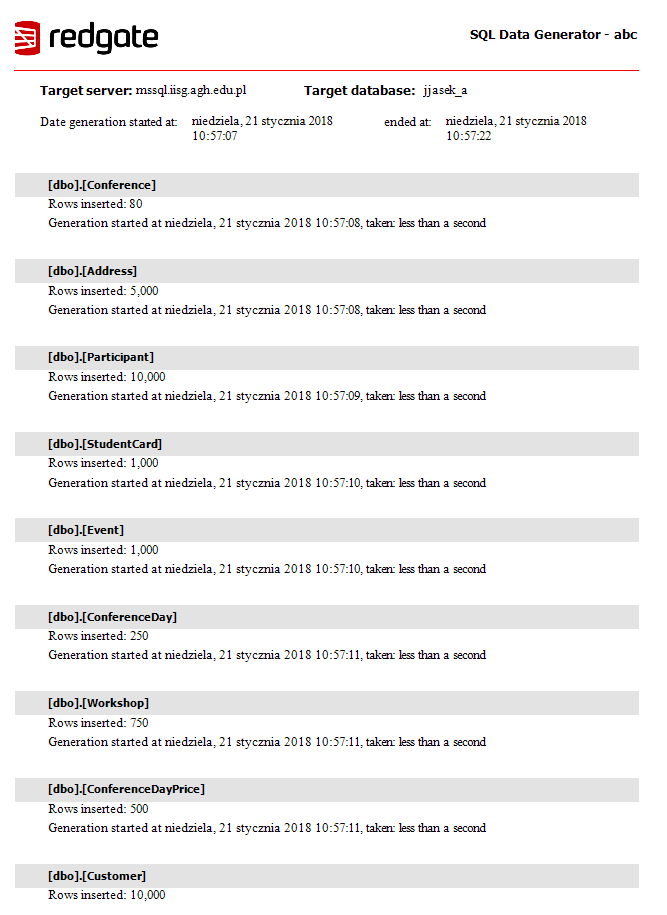
\includegraphics[width=0.9\textwidth]{redgate1}
\end{figure}
\begin{figure}[H]
	\centering
	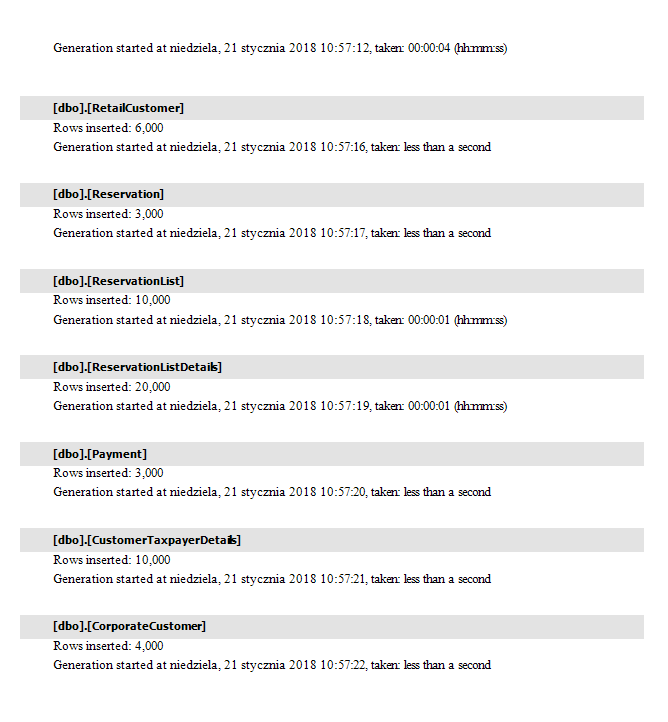
\includegraphics[width=0.9\textwidth]{redgate2}
\end{figure}
\section{Role}
	W systemie wprowadzilibyśmy następujące role:
	\begin{itemize}
		\item companyDatabaseAdmin - administrator bazy danych firmy, który ma dostęp do wszystkich tabel, widoków, funkcji, procedur.
		\item companyWorker - zwykły pracownik firmy, który ma dostęp do bazy danych. Ma dostęp do procedur, widoków i tabel, jednak po części ograniczone tylko do wykonywania SELECT. Aby dodać, zmodyfikować lub usunąć dane, pracownik musi wykonać odpowiednią procedurę.
		\item customer - klient firmy, który ma dostęp do danych z poziomu aplikacji www. Klient może wyświetlać i modyfikować dane swojej rezerwacji, a także sprawdzać stan swoich płatności za pomocą odpowiednich procedur. Klient ma dostęp do niektórych widoków i tabel, ale może je tylko wyświetlić.
		\item participant - uczestnik konferencji, może wyświetlać wydarzenia w których uczestniczy.
	\end{itemize}
\end{document}
